\documentclass[11pt,preprint, authoryear]{elsarticle}

\usepackage{lmodern}
%%%% My spacing
\usepackage{setspace}
\setstretch{1.2}
\DeclareMathSizes{12}{14}{10}{10}

% Wrap around which gives all figures included the [H] command, or places it "here". This can be tedious to code in Rmarkdown.
\usepackage{float}
\let\origfigure\figure
\let\endorigfigure\endfigure
\renewenvironment{figure}[1][2] {
    \expandafter\origfigure\expandafter[H]
} {
    \endorigfigure
}

\let\origtable\table
\let\endorigtable\endtable
\renewenvironment{table}[1][2] {
    \expandafter\origtable\expandafter[H]
} {
    \endorigtable
}


\usepackage{ifxetex,ifluatex}
\usepackage{fixltx2e} % provides \textsubscript
\ifnum 0\ifxetex 1\fi\ifluatex 1\fi=0 % if pdftex
  \usepackage[T1]{fontenc}
  \usepackage[utf8]{inputenc}
\else % if luatex or xelatex
  \ifxetex
    \usepackage{mathspec}
    \usepackage{xltxtra,xunicode}
  \else
    \usepackage{fontspec}
  \fi
  \defaultfontfeatures{Mapping=tex-text,Scale=MatchLowercase}
  \newcommand{\euro}{€}
\fi

\usepackage{amssymb, amsmath, amsthm, amsfonts}

\def\bibsection{\section*{References}} %%% Make "References" appear before bibliography


\usepackage[round]{natbib}

\usepackage{longtable}
\usepackage[margin=2.3cm,bottom=2cm,top=2.5cm, includefoot]{geometry}
\usepackage{fancyhdr}
\usepackage[bottom, hang, flushmargin]{footmisc}
\usepackage{graphicx}
\numberwithin{equation}{section}
\numberwithin{figure}{section}
\numberwithin{table}{section}
\setlength{\parindent}{0cm}
\setlength{\parskip}{1.3ex plus 0.5ex minus 0.3ex}
\usepackage{textcomp}
\renewcommand{\headrulewidth}{0.2pt}
\renewcommand{\footrulewidth}{0.3pt}

\usepackage{array}
\newcolumntype{x}[1]{>{\centering\arraybackslash\hspace{0pt}}p{#1}}

%%%%  Remove the "preprint submitted to" part. Don't worry about this either, it just looks better without it:
\makeatletter
\def\ps@pprintTitle{%
  \let\@oddhead\@empty
  \let\@evenhead\@empty
  \let\@oddfoot\@empty
  \let\@evenfoot\@oddfoot
}
\makeatother

 \def\tightlist{} % This allows for subbullets!

\usepackage{hyperref}
\hypersetup{breaklinks=true,
            bookmarks=true,
            colorlinks=true,
            citecolor=blue,
            urlcolor=blue,
            linkcolor=blue,
            pdfborder={0 0 0}}


% The following packages allow huxtable to work:
\usepackage{siunitx}
\usepackage{multirow}
\usepackage{hhline}
\usepackage{calc}
\usepackage{tabularx}
\usepackage{booktabs}
\usepackage{caption}


\newenvironment{columns}[1][]{}{}

\newenvironment{column}[1]{\begin{minipage}{#1}\ignorespaces}{%
\end{minipage}
\ifhmode\unskip\fi
\aftergroup\useignorespacesandallpars}

\def\useignorespacesandallpars#1\ignorespaces\fi{%
#1\fi\ignorespacesandallpars}

\makeatletter
\def\ignorespacesandallpars{%
  \@ifnextchar\par
    {\expandafter\ignorespacesandallpars\@gobble}%
    {}%
}
\makeatother

\newenvironment{CSLReferences}[2]{%
}

\urlstyle{same}  % don't use monospace font for urls
\setlength{\parindent}{0pt}
\setlength{\parskip}{6pt plus 2pt minus 1pt}
\setlength{\emergencystretch}{3em}  % prevent overfull lines
\setcounter{secnumdepth}{5}

%%% Use protect on footnotes to avoid problems with footnotes in titles
\let\rmarkdownfootnote\footnote%
\def\footnote{\protect\rmarkdownfootnote}
\IfFileExists{upquote.sty}{\usepackage{upquote}}{}

%%% Include extra packages specified by user

%%% Hard setting column skips for reports - this ensures greater consistency and control over the length settings in the document.
%% page layout
%% paragraphs
\setlength{\baselineskip}{12pt plus 0pt minus 0pt}
\setlength{\parskip}{12pt plus 0pt minus 0pt}
\setlength{\parindent}{0pt plus 0pt minus 0pt}
%% floats
\setlength{\floatsep}{12pt plus 0 pt minus 0pt}
\setlength{\textfloatsep}{20pt plus 0pt minus 0pt}
\setlength{\intextsep}{14pt plus 0pt minus 0pt}
\setlength{\dbltextfloatsep}{20pt plus 0pt minus 0pt}
\setlength{\dblfloatsep}{14pt plus 0pt minus 0pt}
%% maths
\setlength{\abovedisplayskip}{12pt plus 0pt minus 0pt}
\setlength{\belowdisplayskip}{12pt plus 0pt minus 0pt}
%% lists
\setlength{\topsep}{10pt plus 0pt minus 0pt}
\setlength{\partopsep}{3pt plus 0pt minus 0pt}
\setlength{\itemsep}{5pt plus 0pt minus 0pt}
\setlength{\labelsep}{8mm plus 0mm minus 0mm}
\setlength{\parsep}{\the\parskip}
\setlength{\listparindent}{\the\parindent}
%% verbatim
\setlength{\fboxsep}{5pt plus 0pt minus 0pt}



\begin{document}



\begin{frontmatter}  %

\title{Predicting Total Auction Values in the Cape Colony}

% Set to FALSE if wanting to remove title (for submission)




\author[Add1]{Tessa Hubble}
\ead{21559953@sun.ac.za}





\address[Add1]{Stellenbosch University, South Africa}


\begin{abstract}
\small{
Predicting total auction values from a Cape Colony auction dataset
between 1720 and 1820.
}
\end{abstract}

\vspace{1cm}





\vspace{0.5cm}

\end{frontmatter}

\setcounter{footnote}{0}



%________________________
% Header and Footers
%%%%%%%%%%%%%%%%%%%%%%%%%%%%%%%%%
\pagestyle{fancy}
\chead{}
\rhead{}
\lfoot{}
\rfoot{\footnotesize Page \thepage}
\lhead{}
%\rfoot{\footnotesize Page \thepage } % "e.g. Page 2"
\cfoot{}

%\setlength\headheight{30pt}
%%%%%%%%%%%%%%%%%%%%%%%%%%%%%%%%%
%________________________

\headsep 35pt % So that header does not go over title




\hypertarget{introduction}{%
\section{\texorpdfstring{Introduction
\label{Introduction}}{Introduction }}\label{introduction}}

Over the first 150 years of the Cape Colony, deceased estate auctions
were an important means of exchange for the burgeoning population
present. The only other means of purchasing goods was through ships that
docked along the coast. From livestock and furniture to slaves, a wide
variety of goods were obtained through auctions. Although auction rolls
from this time period have been transcribed, inconsistent spelling and
errors are pervasive. 30 types of goods have been identified and tagged
throughout the auction rolls. This project aims to use this subset of
goods within auctions to predict total auction values. Focusing on
approximately 1400 auctions between 1720 and 1820, two different machine
learning techniques will be used to predict total auction values. Being
able to assess the total auction value based on a subset of goods can be
an important tool within historical data where there is limited
information. Exploratory data analysis will provide context and support
for the features included in the models. Throughout the exploratory data
analysis and subsequent models, it becomes clear that the number of
slaves, \ldots\ldots. consistently place upward pressure on total
auction values. The performance of a k-nearest neighbours model and
random forest model will be compared to that of a linear regression to
assess accuracy. (give brief results)

\hypertarget{auction-data}{%
\section{Auction data}\label{auction-data}}

Table 1 below provides an example of one auction in 1770. From this
auction roll, one can see the goods sold, the price and the type of good
sold. A buyer\_id column exists as well. Within this column, some names
include titles such as ``de Wede'' (widow) or ``mijnheer'' (mister)
which enables one to determine how many titled men or women attend an
auction. It is clear from this auction that only a few goods are tagged.
The tagged/ subset group of goods will be as features therefore the
accuracy of the machine learning models included may be hampered by
limited presence of these goods across auctions.

\begin{verbatim}
## [1] "\n\n```{=latex}\n \n  \\providecommand{\\huxb}[2]{\\arrayrulecolor[RGB]{#1}\\global\\arrayrulewidth=#2pt}\n  \\providecommand{\\huxvb}[2]{\\color[RGB]{#1}\\vrule width #2pt}\n  \\providecommand{\\huxtpad}[1]{\\rule{0pt}{#1}}\n  \\providecommand{\\huxbpad}[1]{\\rule[-#1]{0pt}{#1}}\n\n\\begin{table}[ht]\n\\begin{centerbox}\n\\begin{threeparttable}\n \\label{tab:Table1}\n\\setlength{\\tabcolsep}{0pt}\n\\begin{tabular}{l l l l l}\n\n\n\\hhline{}\n\\arrayrulecolor{black}\n\n\\multicolumn{1}{!{\\huxvb{0, 0, 0}{0}}l!{\\huxvb{0, 0, 0}{0}}}{\\huxtpad{6pt + 1em}\\raggedright \\hspace{6pt} mooc\\_id \\hspace{6pt}\\huxbpad{6pt}} &\n\\multicolumn{1}{l!{\\huxvb{0, 0, 0}{0}}}{\\huxtpad{6pt + 1em}\\raggedright \\hspace{6pt} purchase\\_id \\hspace{6pt}\\huxbpad{6pt}} &\n\\multicolumn{1}{l!{\\huxvb{0, 0, 0}{0}}}{\\huxtpad{6pt + 1em}\\raggedright \\hspace{6pt} price \\hspace{6pt}\\huxbpad{6pt}} &\n\\multicolumn{1}{l!{\\huxvb{0, 0, 0}{0}}}{\\huxtpad{6pt + 1em}\\raggedright \\hspace{6pt} goods \\hspace{6pt}\\huxbpad{6pt}} &\n\\multicolumn{1}{l!{\\huxvb{0, 0, 0}{0}}}{\\huxtpad{6pt + 1em}\\raggedright \\hspace{6pt} type \\hspace{6pt}\\huxbpad{6pt}} \\tabularnewline[-0.5pt]\n\n\n\\hhline{}\n\\arrayrulecolor{black}\n\n\\multicolumn{1}{!{\\huxvb{0, 0, 0}{0}}l!{\\huxvb{0, 0, 0}{0}}}{\\huxtpad{6pt + 1em}\\raggedright \\hspace{6pt} MOOC10/10.1 \\hspace{6pt}\\huxbpad{6pt}} &\n\\multicolumn{1}{l!{\\huxvb{0, 0, 0}{0}}}{\\huxtpad{6pt + 1em}\\raggedright \\hspace{6pt} MOOC10/10.1/3 \\hspace{6pt}\\huxbpad{6pt}} &\n\\multicolumn{1}{l!{\\huxvb{0, 0, 0}{0}}}{\\huxtpad{6pt + 1em}\\raggedright \\hspace{6pt} 1 \\hspace{6pt}\\huxbpad{6pt}} &\n\\multicolumn{1}{l!{\\huxvb{0, 0, 0}{0}}}{\\huxtpad{6pt + 1em}\\raggedright \\hspace{6pt} 1 porc:ne lampet en schotel en 2 trekpotjes \\hspace{6pt}\\huxbpad{6pt}} &\n\\multicolumn{1}{l!{\\huxvb{0, 0, 0}{0}}}{\\huxtpad{6pt + 1em}\\raggedright \\hspace{6pt} china \\hspace{6pt}\\huxbpad{6pt}} \\tabularnewline[-0.5pt]\n\n\n\\hhline{}\n\\arrayrulecolor{black}\n\n\\multicolumn{1}{!{\\huxvb{0, 0, 0}{0}}l!{\\huxvb{0, 0, 0}{0}}}{\\huxtpad{6pt + 1em}\\raggedright \\hspace{6pt} MOOC10/10.1 \\hspace{6pt}\\huxbpad{6pt}} &\n\\multicolumn{1}{l!{\\huxvb{0, 0, 0}{0}}}{\\huxtpad{6pt + 1em}\\raggedright \\hspace{6pt} MOOC10/10.1/30 \\hspace{6pt}\\huxbpad{6pt}} &\n\\multicolumn{1}{l!{\\huxvb{0, 0, 0}{0}}}{\\huxtpad{6pt + 1em}\\raggedright \\hspace{6pt} 1 \\hspace{6pt}\\huxbpad{6pt}} &\n\\multicolumn{1}{l!{\\huxvb{0, 0, 0}{0}}}{\\huxtpad{6pt + 1em}\\raggedright \\hspace{6pt} 10 handdoeken \\hspace{6pt}\\huxbpad{6pt}} &\n\\multicolumn{1}{l!{\\huxvb{0, 0, 0}{0}}}{\\huxtpad{6pt + 1em}\\raggedright \\hspace{6pt}  \\hspace{6pt}\\huxbpad{6pt}} \\tabularnewline[-0.5pt]\n\n\n\\hhline{}\n\\arrayrulecolor{black}\n\n\\multicolumn{1}{!{\\huxvb{0, 0, 0}{0}}l!{\\huxvb{0, 0, 0}{0}}}{\\huxtpad{6pt + 1em}\\raggedright \\hspace{6pt} MOOC10/10.1 \\hspace{6pt}\\huxbpad{6pt}} &\n\\multicolumn{1}{l!{\\huxvb{0, 0, 0}{0}}}{\\huxtpad{6pt + 1em}\\raggedright \\hspace{6pt} MOOC10/10.1/37 \\hspace{6pt}\\huxbpad{6pt}} &\n\\multicolumn{1}{l!{\\huxvb{0, 0, 0}{0}}}{\\huxtpad{6pt + 1em}\\raggedright \\hspace{6pt} 2 \\hspace{6pt}\\huxbpad{6pt}} &\n\\multicolumn{1}{l!{\\huxvb{0, 0, 0}{0}}}{\\huxtpad{6pt + 1em}\\raggedright \\hspace{6pt} 3 sprijen \\hspace{6pt}\\huxbpad{6pt}} &\n\\multicolumn{1}{l!{\\huxvb{0, 0, 0}{0}}}{\\huxtpad{6pt + 1em}\\raggedright \\hspace{6pt}  \\hspace{6pt}\\huxbpad{6pt}} \\tabularnewline[-0.5pt]\n\n\n\\hhline{}\n\\arrayrulecolor{black}\n\n\\multicolumn{1}{!{\\huxvb{0, 0, 0}{0}}l!{\\huxvb{0, 0, 0}{0}}}{\\huxtpad{6pt + 1em}\\raggedright \\hspace{6pt} MOOC10/10.1 \\hspace{6pt}\\huxbpad{6pt}} &\n\\multicolumn{1}{l!{\\huxvb{0, 0, 0}{0}}}{\\huxtpad{6pt + 1em}\\raggedright \\hspace{6pt} MOOC10/10.1/52 \\hspace{6pt}\\huxbpad{6pt}} &\n\\multicolumn{1}{l!{\\huxvb{0, 0, 0}{0}}}{\\huxtpad{6pt + 1em}\\raggedright \\hspace{6pt} 2 \\hspace{6pt}\\huxbpad{6pt}} &\n\\multicolumn{1}{l!{\\huxvb{0, 0, 0}{0}}}{\\huxtpad{6pt + 1em}\\raggedright \\hspace{6pt} 1 ledige kist en 1 stoel \\hspace{6pt}\\huxbpad{6pt}} &\n\\multicolumn{1}{l!{\\huxvb{0, 0, 0}{0}}}{\\huxtpad{6pt + 1em}\\raggedright \\hspace{6pt} chairs \\hspace{6pt}\\huxbpad{6pt}} \\tabularnewline[-0.5pt]\n\n\n\\hhline{}\n\\arrayrulecolor{black}\n\n\\multicolumn{1}{!{\\huxvb{0, 0, 0}{0}}l!{\\huxvb{0, 0, 0}{0}}}{\\huxtpad{6pt + 1em}\\raggedright \\hspace{6pt} MOOC10/10.1 \\hspace{6pt}\\huxbpad{6pt}} &\n\\multicolumn{1}{l!{\\huxvb{0, 0, 0}{0}}}{\\huxtpad{6pt + 1em}\\raggedright \\hspace{6pt} MOOC10/10.1/29 \\hspace{6pt}\\huxbpad{6pt}} &\n\\multicolumn{1}{l!{\\huxvb{0, 0, 0}{0}}}{\\huxtpad{6pt + 1em}\\raggedright \\hspace{6pt} 3 \\hspace{6pt}\\huxbpad{6pt}} &\n\\multicolumn{1}{l!{\\huxvb{0, 0, 0}{0}}}{\\huxtpad{6pt + 1em}\\raggedright \\hspace{6pt} 14 sloopen in zoort \\hspace{6pt}\\huxbpad{6pt}} &\n\\multicolumn{1}{l!{\\huxvb{0, 0, 0}{0}}}{\\huxtpad{6pt + 1em}\\raggedright \\hspace{6pt}  \\hspace{6pt}\\huxbpad{6pt}} \\tabularnewline[-0.5pt]\n\n\n\\hhline{}\n\\arrayrulecolor{black}\n\n\\multicolumn{1}{!{\\huxvb{0, 0, 0}{0}}l!{\\huxvb{0, 0, 0}{0}}}{\\huxtpad{6pt + 1em}\\raggedright \\hspace{6pt} MOOC10/10.1 \\hspace{6pt}\\huxbpad{6pt}} &\n\\multicolumn{1}{l!{\\huxvb{0, 0, 0}{0}}}{\\huxtpad{6pt + 1em}\\raggedright \\hspace{6pt} MOOC10/10.1/55 \\hspace{6pt}\\huxbpad{6pt}} &\n\\multicolumn{1}{l!{\\huxvb{0, 0, 0}{0}}}{\\huxtpad{6pt + 1em}\\raggedright \\hspace{6pt} 4 \\hspace{6pt}\\huxbpad{6pt}} &\n\\multicolumn{1}{l!{\\huxvb{0, 0, 0}{0}}}{\\huxtpad{6pt + 1em}\\raggedright \\hspace{6pt} 4 sacken \\hspace{6pt}\\huxbpad{6pt}} &\n\\multicolumn{1}{l!{\\huxvb{0, 0, 0}{0}}}{\\huxtpad{6pt + 1em}\\raggedright \\hspace{6pt}  \\hspace{6pt}\\huxbpad{6pt}} \\tabularnewline[-0.5pt]\n\n\n\\hhline{}\n\\arrayrulecolor{black}\n\n\\multicolumn{1}{!{\\huxvb{0, 0, 0}{0}}l!{\\huxvb{0, 0, 0}{0}}}{\\huxtpad{6pt + 1em}\\raggedright \\hspace{6pt} MOOC10/10.1 \\hspace{6pt}\\huxbpad{6pt}} &\n\\multicolumn{1}{l!{\\huxvb{0, 0, 0}{0}}}{\\huxtpad{6pt + 1em}\\raggedright \\hspace{6pt} MOOC10/10.1/57 \\hspace{6pt}\\huxbpad{6pt}} &\n\\multicolumn{1}{l!{\\huxvb{0, 0, 0}{0}}}{\\huxtpad{6pt + 1em}\\raggedright \\hspace{6pt} 6 \\hspace{6pt}\\huxbpad{6pt}} &\n\\multicolumn{1}{l!{\\huxvb{0, 0, 0}{0}}}{\\huxtpad{6pt + 1em}\\raggedright \\hspace{6pt} 7 cabaijen \\hspace{6pt}\\huxbpad{6pt}} &\n\\multicolumn{1}{l!{\\huxvb{0, 0, 0}{0}}}{\\huxtpad{6pt + 1em}\\raggedright \\hspace{6pt}  \\hspace{6pt}\\huxbpad{6pt}} \\tabularnewline[-0.5pt]\n\n\n\\hhline{}\n\\arrayrulecolor{black}\n\n\\multicolumn{1}{!{\\huxvb{0, 0, 0}{0}}l!{\\huxvb{0, 0, 0}{0}}}{\\huxtpad{6pt + 1em}\\raggedright \\hspace{6pt} MOOC10/10.1 \\hspace{6pt}\\huxbpad{6pt}} &\n\\multicolumn{1}{l!{\\huxvb{0, 0, 0}{0}}}{\\huxtpad{6pt + 1em}\\raggedright \\hspace{6pt} MOOC10/10.1/60 \\hspace{6pt}\\huxbpad{6pt}} &\n\\multicolumn{1}{l!{\\huxvb{0, 0, 0}{0}}}{\\huxtpad{6pt + 1em}\\raggedright \\hspace{6pt} 10 \\hspace{6pt}\\huxbpad{6pt}} &\n\\multicolumn{1}{l!{\\huxvb{0, 0, 0}{0}}}{\\huxtpad{6pt + 1em}\\raggedright \\hspace{6pt} 5 borstrocken, 15 voorschooden, 28 neusdoeken, 12 nagtcapjes, 15 p:r cousen, 12 p:r vr: handschoenen, 6 p:r mofjes, 4 p:r lubben \\hspace{6pt}\\huxbpad{6pt}} &\n\\multicolumn{1}{l!{\\huxvb{0, 0, 0}{0}}}{\\huxtpad{6pt + 1em}\\raggedright \\hspace{6pt}  \\hspace{6pt}\\huxbpad{6pt}} \\tabularnewline[-0.5pt]\n\n\n\\hhline{}\n\\arrayrulecolor{black}\n\n\\multicolumn{1}{!{\\huxvb{0, 0, 0}{0}}l!{\\huxvb{0, 0, 0}{0}}}{\\huxtpad{6pt + 1em}\\raggedright \\hspace{6pt} MOOC10/10.1 \\hspace{6pt}\\huxbpad{6pt}} &\n\\multicolumn{1}{l!{\\huxvb{0, 0, 0}{0}}}{\\huxtpad{6pt + 1em}\\raggedright \\hspace{6pt} MOOC10/10.1/54 \\hspace{6pt}\\huxbpad{6pt}} &\n\\multicolumn{1}{l!{\\huxvb{0, 0, 0}{0}}}{\\huxtpad{6pt + 1em}\\raggedright \\hspace{6pt} 14 \\hspace{6pt}\\huxbpad{6pt}} &\n\\multicolumn{1}{l!{\\huxvb{0, 0, 0}{0}}}{\\huxtpad{6pt + 1em}\\raggedright \\hspace{6pt} 9 vrouw gonnen \\hspace{6pt}\\huxbpad{6pt}} &\n\\multicolumn{1}{l!{\\huxvb{0, 0, 0}{0}}}{\\huxtpad{6pt + 1em}\\raggedright \\hspace{6pt}  \\hspace{6pt}\\huxbpad{6pt}} \\tabularnewline[-0.5pt]\n\n\n\\hhline{}\n\\arrayrulecolor{black}\n\n\\multicolumn{1}{!{\\huxvb{0, 0, 0}{0}}l!{\\huxvb{0, 0, 0}{0}}}{\\huxtpad{6pt + 1em}\\raggedright \\hspace{6pt} MOOC10/10.1 \\hspace{6pt}\\huxbpad{6pt}} &\n\\multicolumn{1}{l!{\\huxvb{0, 0, 0}{0}}}{\\huxtpad{6pt + 1em}\\raggedright \\hspace{6pt} MOOC10/10.1/58 \\hspace{6pt}\\huxbpad{6pt}} &\n\\multicolumn{1}{l!{\\huxvb{0, 0, 0}{0}}}{\\huxtpad{6pt + 1em}\\raggedright \\hspace{6pt} 15 \\hspace{6pt}\\huxbpad{6pt}} &\n\\multicolumn{1}{l!{\\huxvb{0, 0, 0}{0}}}{\\huxtpad{6pt + 1em}\\raggedright \\hspace{6pt} 21 rokken \\hspace{6pt}\\huxbpad{6pt}} &\n\\multicolumn{1}{l!{\\huxvb{0, 0, 0}{0}}}{\\huxtpad{6pt + 1em}\\raggedright \\hspace{6pt}  \\hspace{6pt}\\huxbpad{6pt}} \\tabularnewline[-0.5pt]\n\n\n\\hhline{}\n\\arrayrulecolor{black}\n\n\\multicolumn{1}{!{\\huxvb{0, 0, 0}{0}}l!{\\huxvb{0, 0, 0}{0}}}{\\huxtpad{6pt + 1em}\\raggedright \\hspace{6pt} MOOC10/10.1 \\hspace{6pt}\\huxbpad{6pt}} &\n\\multicolumn{1}{l!{\\huxvb{0, 0, 0}{0}}}{\\huxtpad{6pt + 1em}\\raggedright \\hspace{6pt} MOOC10/10.1/28 \\hspace{6pt}\\huxbpad{6pt}} &\n\\multicolumn{1}{l!{\\huxvb{0, 0, 0}{0}}}{\\huxtpad{6pt + 1em}\\raggedright \\hspace{6pt} 1.1 \\hspace{6pt}\\huxbpad{6pt}} &\n\\multicolumn{1}{l!{\\huxvb{0, 0, 0}{0}}}{\\huxtpad{6pt + 1em}\\raggedright \\hspace{6pt} 16 sloopen in zoort \\hspace{6pt}\\huxbpad{6pt}} &\n\\multicolumn{1}{l!{\\huxvb{0, 0, 0}{0}}}{\\huxtpad{6pt + 1em}\\raggedright \\hspace{6pt}  \\hspace{6pt}\\huxbpad{6pt}} \\tabularnewline[-0.5pt]\n\n\n\\hhline{}\n\\arrayrulecolor{black}\n\n\\multicolumn{1}{!{\\huxvb{0, 0, 0}{0}}l!{\\huxvb{0, 0, 0}{0}}}{\\huxtpad{6pt + 1em}\\raggedright \\hspace{6pt} MOOC10/10.1 \\hspace{6pt}\\huxbpad{6pt}} &\n\\multicolumn{1}{l!{\\huxvb{0, 0, 0}{0}}}{\\huxtpad{6pt + 1em}\\raggedright \\hspace{6pt} MOOC10/10.1/53 \\hspace{6pt}\\huxbpad{6pt}} &\n\\multicolumn{1}{l!{\\huxvb{0, 0, 0}{0}}}{\\huxtpad{6pt + 1em}\\raggedright \\hspace{6pt} 1.1 \\hspace{6pt}\\huxbpad{6pt}} &\n\\multicolumn{1}{l!{\\huxvb{0, 0, 0}{0}}}{\\huxtpad{6pt + 1em}\\raggedright \\hspace{6pt} 1 ledige kist \\hspace{6pt}\\huxbpad{6pt}} &\n\\multicolumn{1}{l!{\\huxvb{0, 0, 0}{0}}}{\\huxtpad{6pt + 1em}\\raggedright \\hspace{6pt}  \\hspace{6pt}\\huxbpad{6pt}} \\tabularnewline[-0.5pt]\n\n\n\\hhline{}\n\\arrayrulecolor{black}\n\n\\multicolumn{1}{!{\\huxvb{0, 0, 0}{0}}l!{\\huxvb{0, 0, 0}{0}}}{\\huxtpad{6pt + 1em}\\raggedright \\hspace{6pt} MOOC10/10.1 \\hspace{6pt}\\huxbpad{6pt}} &\n\\multicolumn{1}{l!{\\huxvb{0, 0, 0}{0}}}{\\huxtpad{6pt + 1em}\\raggedright \\hspace{6pt} MOOC10/10.1/7 \\hspace{6pt}\\huxbpad{6pt}} &\n\\multicolumn{1}{l!{\\huxvb{0, 0, 0}{0}}}{\\huxtpad{6pt + 1em}\\raggedright \\hspace{6pt} 2.1 \\hspace{6pt}\\huxbpad{6pt}} &\n\\multicolumn{1}{l!{\\huxvb{0, 0, 0}{0}}}{\\huxtpad{6pt + 1em}\\raggedright \\hspace{6pt} 2 copere strijkijsers \\hspace{6pt}\\huxbpad{6pt}} &\n\\multicolumn{1}{l!{\\huxvb{0, 0, 0}{0}}}{\\huxtpad{6pt + 1em}\\raggedright \\hspace{6pt} irons \\hspace{6pt}\\huxbpad{6pt}} \\tabularnewline[-0.5pt]\n\n\n\\hhline{}\n\\arrayrulecolor{black}\n\n\\multicolumn{1}{!{\\huxvb{0, 0, 0}{0}}l!{\\huxvb{0, 0, 0}{0}}}{\\huxtpad{6pt + 1em}\\raggedright \\hspace{6pt} MOOC10/10.1 \\hspace{6pt}\\huxbpad{6pt}} &\n\\multicolumn{1}{l!{\\huxvb{0, 0, 0}{0}}}{\\huxtpad{6pt + 1em}\\raggedright \\hspace{6pt} MOOC10/10.1/11 \\hspace{6pt}\\huxbpad{6pt}} &\n\\multicolumn{1}{l!{\\huxvb{0, 0, 0}{0}}}{\\huxtpad{6pt + 1em}\\raggedright \\hspace{6pt} 2.1 \\hspace{6pt}\\huxbpad{6pt}} &\n\\multicolumn{1}{l!{\\huxvb{0, 0, 0}{0}}}{\\huxtpad{6pt + 1em}\\raggedright \\hspace{6pt} 1 casje met thee en 1 bijbel \\hspace{6pt}\\huxbpad{6pt}} &\n\\multicolumn{1}{l!{\\huxvb{0, 0, 0}{0}}}{\\huxtpad{6pt + 1em}\\raggedright \\hspace{6pt} books \\hspace{6pt}\\huxbpad{6pt}} \\tabularnewline[-0.5pt]\n\n\n\\hhline{}\n\\arrayrulecolor{black}\n\n\\multicolumn{1}{!{\\huxvb{0, 0, 0}{0}}l!{\\huxvb{0, 0, 0}{0}}}{\\huxtpad{6pt + 1em}\\raggedright \\hspace{6pt} MOOC10/10.1 \\hspace{6pt}\\huxbpad{6pt}} &\n\\multicolumn{1}{l!{\\huxvb{0, 0, 0}{0}}}{\\huxtpad{6pt + 1em}\\raggedright \\hspace{6pt} MOOC10/10.1/27 \\hspace{6pt}\\huxbpad{6pt}} &\n\\multicolumn{1}{l!{\\huxvb{0, 0, 0}{0}}}{\\huxtpad{6pt + 1em}\\raggedright \\hspace{6pt} 2.1 \\hspace{6pt}\\huxbpad{6pt}} &\n\\multicolumn{1}{l!{\\huxvb{0, 0, 0}{0}}}{\\huxtpad{6pt + 1em}\\raggedright \\hspace{6pt} 12 sloopen in zoort \\hspace{6pt}\\huxbpad{6pt}} &\n\\multicolumn{1}{l!{\\huxvb{0, 0, 0}{0}}}{\\huxtpad{6pt + 1em}\\raggedright \\hspace{6pt}  \\hspace{6pt}\\huxbpad{6pt}} \\tabularnewline[-0.5pt]\n\n\n\\hhline{}\n\\arrayrulecolor{black}\n\n\\multicolumn{1}{!{\\huxvb{0, 0, 0}{0}}l!{\\huxvb{0, 0, 0}{0}}}{\\huxtpad{6pt + 1em}\\raggedright \\hspace{6pt} MOOC10/10.1 \\hspace{6pt}\\huxbpad{6pt}} &\n\\multicolumn{1}{l!{\\huxvb{0, 0, 0}{0}}}{\\huxtpad{6pt + 1em}\\raggedright \\hspace{6pt} MOOC10/10.1/36 \\hspace{6pt}\\huxbpad{6pt}} &\n\\multicolumn{1}{l!{\\huxvb{0, 0, 0}{0}}}{\\huxtpad{6pt + 1em}\\raggedright \\hspace{6pt} 2.1 \\hspace{6pt}\\huxbpad{6pt}} &\n\\multicolumn{1}{l!{\\huxvb{0, 0, 0}{0}}}{\\huxtpad{6pt + 1em}\\raggedright \\hspace{6pt} 1 partij garen en papier \\hspace{6pt}\\huxbpad{6pt}} &\n\\multicolumn{1}{l!{\\huxvb{0, 0, 0}{0}}}{\\huxtpad{6pt + 1em}\\raggedright \\hspace{6pt}  \\hspace{6pt}\\huxbpad{6pt}} \\tabularnewline[-0.5pt]\n\n\n\\hhline{}\n\\arrayrulecolor{black}\n\n\\multicolumn{1}{!{\\huxvb{0, 0, 0}{0}}l!{\\huxvb{0, 0, 0}{0}}}{\\huxtpad{6pt + 1em}\\raggedright \\hspace{6pt} MOOC10/10.1 \\hspace{6pt}\\huxbpad{6pt}} &\n\\multicolumn{1}{l!{\\huxvb{0, 0, 0}{0}}}{\\huxtpad{6pt + 1em}\\raggedright \\hspace{6pt} MOOC10/10.1/12 \\hspace{6pt}\\huxbpad{6pt}} &\n\\multicolumn{1}{l!{\\huxvb{0, 0, 0}{0}}}{\\huxtpad{6pt + 1em}\\raggedright \\hspace{6pt} 3.1 \\hspace{6pt}\\huxbpad{6pt}} &\n\\multicolumn{1}{l!{\\huxvb{0, 0, 0}{0}}}{\\huxtpad{6pt + 1em}\\raggedright \\hspace{6pt} 6 kussens \\hspace{6pt}\\huxbpad{6pt}} &\n\\multicolumn{1}{l!{\\huxvb{0, 0, 0}{0}}}{\\huxtpad{6pt + 1em}\\raggedright \\hspace{6pt}  \\hspace{6pt}\\huxbpad{6pt}} \\tabularnewline[-0.5pt]\n\n\n\\hhline{}\n\\arrayrulecolor{black}\n\n\\multicolumn{1}{!{\\huxvb{0, 0, 0}{0}}l!{\\huxvb{0, 0, 0}{0}}}{\\huxtpad{6pt + 1em}\\raggedright \\hspace{6pt} MOOC10/10.1 \\hspace{6pt}\\huxbpad{6pt}} &\n\\multicolumn{1}{l!{\\huxvb{0, 0, 0}{0}}}{\\huxtpad{6pt + 1em}\\raggedright \\hspace{6pt} MOOC10/10.1/43 \\hspace{6pt}\\huxbpad{6pt}} &\n\\multicolumn{1}{l!{\\huxvb{0, 0, 0}{0}}}{\\huxtpad{6pt + 1em}\\raggedright \\hspace{6pt} 9.1 \\hspace{6pt}\\huxbpad{6pt}} &\n\\multicolumn{1}{l!{\\huxvb{0, 0, 0}{0}}}{\\huxtpad{6pt + 1em}\\raggedright \\hspace{6pt} 4 silvere leepels \\hspace{6pt}\\huxbpad{6pt}} &\n\\multicolumn{1}{l!{\\huxvb{0, 0, 0}{0}}}{\\huxtpad{6pt + 1em}\\raggedright \\hspace{6pt} utensils \\hspace{6pt}\\huxbpad{6pt}} \\tabularnewline[-0.5pt]\n\n\n\\hhline{}\n\\arrayrulecolor{black}\n\n\\multicolumn{1}{!{\\huxvb{0, 0, 0}{0}}l!{\\huxvb{0, 0, 0}{0}}}{\\huxtpad{6pt + 1em}\\raggedright \\hspace{6pt} MOOC10/10.1 \\hspace{6pt}\\huxbpad{6pt}} &\n\\multicolumn{1}{l!{\\huxvb{0, 0, 0}{0}}}{\\huxtpad{6pt + 1em}\\raggedright \\hspace{6pt} MOOC10/10.1/48 \\hspace{6pt}\\huxbpad{6pt}} &\n\\multicolumn{1}{l!{\\huxvb{0, 0, 0}{0}}}{\\huxtpad{6pt + 1em}\\raggedright \\hspace{6pt} 2.2 \\hspace{6pt}\\huxbpad{6pt}} &\n\\multicolumn{1}{l!{\\huxvb{0, 0, 0}{0}}}{\\huxtpad{6pt + 1em}\\raggedright \\hspace{6pt} 1 goude ring met 1 rode steen \\hspace{6pt}\\huxbpad{6pt}} &\n\\multicolumn{1}{l!{\\huxvb{0, 0, 0}{0}}}{\\huxtpad{6pt + 1em}\\raggedright \\hspace{6pt} jewlery \\hspace{6pt}\\huxbpad{6pt}} \\tabularnewline[-0.5pt]\n\n\n\\hhline{}\n\\arrayrulecolor{black}\n\n\\multicolumn{1}{!{\\huxvb{0, 0, 0}{0}}l!{\\huxvb{0, 0, 0}{0}}}{\\huxtpad{6pt + 1em}\\raggedright \\hspace{6pt} MOOC10/10.1 \\hspace{6pt}\\huxbpad{6pt}} &\n\\multicolumn{1}{l!{\\huxvb{0, 0, 0}{0}}}{\\huxtpad{6pt + 1em}\\raggedright \\hspace{6pt} MOOC10/10.1/13 \\hspace{6pt}\\huxbpad{6pt}} &\n\\multicolumn{1}{l!{\\huxvb{0, 0, 0}{0}}}{\\huxtpad{6pt + 1em}\\raggedright \\hspace{6pt} 3.2 \\hspace{6pt}\\huxbpad{6pt}} &\n\\multicolumn{1}{l!{\\huxvb{0, 0, 0}{0}}}{\\huxtpad{6pt + 1em}\\raggedright \\hspace{6pt} 5 kussens \\hspace{6pt}\\huxbpad{6pt}} &\n\\multicolumn{1}{l!{\\huxvb{0, 0, 0}{0}}}{\\huxtpad{6pt + 1em}\\raggedright \\hspace{6pt}  \\hspace{6pt}\\huxbpad{6pt}} \\tabularnewline[-0.5pt]\n\n\n\\hhline{}\n\\arrayrulecolor{black}\n\n\\multicolumn{1}{!{\\huxvb{0, 0, 0}{0}}l!{\\huxvb{0, 0, 0}{0}}}{\\huxtpad{6pt + 1em}\\raggedright \\hspace{6pt} MOOC10/10.1 \\hspace{6pt}\\huxbpad{6pt}} &\n\\multicolumn{1}{l!{\\huxvb{0, 0, 0}{0}}}{\\huxtpad{6pt + 1em}\\raggedright \\hspace{6pt} MOOC10/10.1/49 \\hspace{6pt}\\huxbpad{6pt}} &\n\\multicolumn{1}{l!{\\huxvb{0, 0, 0}{0}}}{\\huxtpad{6pt + 1em}\\raggedright \\hspace{6pt} 3.2 \\hspace{6pt}\\huxbpad{6pt}} &\n\\multicolumn{1}{l!{\\huxvb{0, 0, 0}{0}}}{\\huxtpad{6pt + 1em}\\raggedright \\hspace{6pt} 1 p:r goude oorcrabbetjes \\hspace{6pt}\\huxbpad{6pt}} &\n\\multicolumn{1}{l!{\\huxvb{0, 0, 0}{0}}}{\\huxtpad{6pt + 1em}\\raggedright \\hspace{6pt} jewlery \\hspace{6pt}\\huxbpad{6pt}} \\tabularnewline[-0.5pt]\n\n\n\\hhline{}\n\\arrayrulecolor{black}\n\n\\multicolumn{1}{!{\\huxvb{0, 0, 0}{0}}l!{\\huxvb{0, 0, 0}{0}}}{\\huxtpad{6pt + 1em}\\raggedright \\hspace{6pt} MOOC10/10.1 \\hspace{6pt}\\huxbpad{6pt}} &\n\\multicolumn{1}{l!{\\huxvb{0, 0, 0}{0}}}{\\huxtpad{6pt + 1em}\\raggedright \\hspace{6pt} MOOC10/10.1/15 \\hspace{6pt}\\huxbpad{6pt}} &\n\\multicolumn{1}{l!{\\huxvb{0, 0, 0}{0}}}{\\huxtpad{6pt + 1em}\\raggedright \\hspace{6pt} 5.2 \\hspace{6pt}\\huxbpad{6pt}} &\n\\multicolumn{1}{l!{\\huxvb{0, 0, 0}{0}}}{\\huxtpad{6pt + 1em}\\raggedright \\hspace{6pt} 1 bijbel en 1 nagtmaalboek met silvere beslag en 4 boeken \\hspace{6pt}\\huxbpad{6pt}} &\n\\multicolumn{1}{l!{\\huxvb{0, 0, 0}{0}}}{\\huxtpad{6pt + 1em}\\raggedright \\hspace{6pt} books \\hspace{6pt}\\huxbpad{6pt}} \\tabularnewline[-0.5pt]\n\n\n\\hhline{}\n\\arrayrulecolor{black}\n\n\\multicolumn{1}{!{\\huxvb{0, 0, 0}{0}}l!{\\huxvb{0, 0, 0}{0}}}{\\huxtpad{6pt + 1em}\\raggedright \\hspace{6pt} MOOC10/10.1 \\hspace{6pt}\\huxbpad{6pt}} &\n\\multicolumn{1}{l!{\\huxvb{0, 0, 0}{0}}}{\\huxtpad{6pt + 1em}\\raggedright \\hspace{6pt} MOOC10/10.1/15 \\hspace{6pt}\\huxbpad{6pt}} &\n\\multicolumn{1}{l!{\\huxvb{0, 0, 0}{0}}}{\\huxtpad{6pt + 1em}\\raggedright \\hspace{6pt} 5.2 \\hspace{6pt}\\huxbpad{6pt}} &\n\\multicolumn{1}{l!{\\huxvb{0, 0, 0}{0}}}{\\huxtpad{6pt + 1em}\\raggedright \\hspace{6pt} 1 bijbel en 1 nagtmaalboek met silvere beslag en 4 boeken \\hspace{6pt}\\huxbpad{6pt}} &\n\\multicolumn{1}{l!{\\huxvb{0, 0, 0}{0}}}{\\huxtpad{6pt + 1em}\\raggedright \\hspace{6pt} books \\hspace{6pt}\\huxbpad{6pt}} \\tabularnewline[-0.5pt]\n\n\n\\hhline{}\n\\arrayrulecolor{black}\n\n\\multicolumn{1}{!{\\huxvb{0, 0, 0}{0}}l!{\\huxvb{0, 0, 0}{0}}}{\\huxtpad{6pt + 1em}\\raggedright \\hspace{6pt} MOOC10/10.1 \\hspace{6pt}\\huxbpad{6pt}} &\n\\multicolumn{1}{l!{\\huxvb{0, 0, 0}{0}}}{\\huxtpad{6pt + 1em}\\raggedright \\hspace{6pt} MOOC10/10.1/42 \\hspace{6pt}\\huxbpad{6pt}} &\n\\multicolumn{1}{l!{\\huxvb{0, 0, 0}{0}}}{\\huxtpad{6pt + 1em}\\raggedright \\hspace{6pt} 6.2 \\hspace{6pt}\\huxbpad{6pt}} &\n\\multicolumn{1}{l!{\\huxvb{0, 0, 0}{0}}}{\\huxtpad{6pt + 1em}\\raggedright \\hspace{6pt} 1 lap wit linnen en 4 neusdoeken \\hspace{6pt}\\huxbpad{6pt}} &\n\\multicolumn{1}{l!{\\huxvb{0, 0, 0}{0}}}{\\huxtpad{6pt + 1em}\\raggedright \\hspace{6pt}  \\hspace{6pt}\\huxbpad{6pt}} \\tabularnewline[-0.5pt]\n\n\n\\hhline{}\n\\arrayrulecolor{black}\n\n\\multicolumn{1}{!{\\huxvb{0, 0, 0}{0}}l!{\\huxvb{0, 0, 0}{0}}}{\\huxtpad{6pt + 1em}\\raggedright \\hspace{6pt} MOOC10/10.1 \\hspace{6pt}\\huxbpad{6pt}} &\n\\multicolumn{1}{l!{\\huxvb{0, 0, 0}{0}}}{\\huxtpad{6pt + 1em}\\raggedright \\hspace{6pt} MOOC10/10.1/40 \\hspace{6pt}\\huxbpad{6pt}} &\n\\multicolumn{1}{l!{\\huxvb{0, 0, 0}{0}}}{\\huxtpad{6pt + 1em}\\raggedright \\hspace{6pt} 7.2 \\hspace{6pt}\\huxbpad{6pt}} &\n\\multicolumn{1}{l!{\\huxvb{0, 0, 0}{0}}}{\\huxtpad{6pt + 1em}\\raggedright \\hspace{6pt} 1 stuk wit linnen \\hspace{6pt}\\huxbpad{6pt}} &\n\\multicolumn{1}{l!{\\huxvb{0, 0, 0}{0}}}{\\huxtpad{6pt + 1em}\\raggedright \\hspace{6pt}  \\hspace{6pt}\\huxbpad{6pt}} \\tabularnewline[-0.5pt]\n\n\n\\hhline{}\n\\arrayrulecolor{black}\n\n\\multicolumn{1}{!{\\huxvb{0, 0, 0}{0}}l!{\\huxvb{0, 0, 0}{0}}}{\\huxtpad{6pt + 1em}\\raggedright \\hspace{6pt} MOOC10/10.1 \\hspace{6pt}\\huxbpad{6pt}} &\n\\multicolumn{1}{l!{\\huxvb{0, 0, 0}{0}}}{\\huxtpad{6pt + 1em}\\raggedright \\hspace{6pt} MOOC10/10.1/4 \\hspace{6pt}\\huxbpad{6pt}} &\n\\multicolumn{1}{l!{\\huxvb{0, 0, 0}{0}}}{\\huxtpad{6pt + 1em}\\raggedright \\hspace{6pt} 0.3 \\hspace{6pt}\\huxbpad{6pt}} &\n\\multicolumn{1}{l!{\\huxvb{0, 0, 0}{0}}}{\\huxtpad{6pt + 1em}\\raggedright \\hspace{6pt} 1 partij porc:n \\hspace{6pt}\\huxbpad{6pt}} &\n\\multicolumn{1}{l!{\\huxvb{0, 0, 0}{0}}}{\\huxtpad{6pt + 1em}\\raggedright \\hspace{6pt} china \\hspace{6pt}\\huxbpad{6pt}} \\tabularnewline[-0.5pt]\n\n\n\\hhline{}\n\\arrayrulecolor{black}\n\n\\multicolumn{1}{!{\\huxvb{0, 0, 0}{0}}l!{\\huxvb{0, 0, 0}{0}}}{\\huxtpad{6pt + 1em}\\raggedright \\hspace{6pt} MOOC10/10.1 \\hspace{6pt}\\huxbpad{6pt}} &\n\\multicolumn{1}{l!{\\huxvb{0, 0, 0}{0}}}{\\huxtpad{6pt + 1em}\\raggedright \\hspace{6pt} MOOC10/10.1/25 \\hspace{6pt}\\huxbpad{6pt}} &\n\\multicolumn{1}{l!{\\huxvb{0, 0, 0}{0}}}{\\huxtpad{6pt + 1em}\\raggedright \\hspace{6pt} 2.3 \\hspace{6pt}\\huxbpad{6pt}} &\n\\multicolumn{1}{l!{\\huxvb{0, 0, 0}{0}}}{\\huxtpad{6pt + 1em}\\raggedright \\hspace{6pt} 12 sloopen in zoort \\hspace{6pt}\\huxbpad{6pt}} &\n\\multicolumn{1}{l!{\\huxvb{0, 0, 0}{0}}}{\\huxtpad{6pt + 1em}\\raggedright \\hspace{6pt}  \\hspace{6pt}\\huxbpad{6pt}} \\tabularnewline[-0.5pt]\n\n\n\\hhline{}\n\\arrayrulecolor{black}\n\n\\multicolumn{1}{!{\\huxvb{0, 0, 0}{0}}l!{\\huxvb{0, 0, 0}{0}}}{\\huxtpad{6pt + 1em}\\raggedright \\hspace{6pt} MOOC10/10.1 \\hspace{6pt}\\huxbpad{6pt}} &\n\\multicolumn{1}{l!{\\huxvb{0, 0, 0}{0}}}{\\huxtpad{6pt + 1em}\\raggedright \\hspace{6pt} MOOC10/10.1/26 \\hspace{6pt}\\huxbpad{6pt}} &\n\\multicolumn{1}{l!{\\huxvb{0, 0, 0}{0}}}{\\huxtpad{6pt + 1em}\\raggedright \\hspace{6pt} 2.3 \\hspace{6pt}\\huxbpad{6pt}} &\n\\multicolumn{1}{l!{\\huxvb{0, 0, 0}{0}}}{\\huxtpad{6pt + 1em}\\raggedright \\hspace{6pt} 12 sloopen in zoort \\hspace{6pt}\\huxbpad{6pt}} &\n\\multicolumn{1}{l!{\\huxvb{0, 0, 0}{0}}}{\\huxtpad{6pt + 1em}\\raggedright \\hspace{6pt}  \\hspace{6pt}\\huxbpad{6pt}} \\tabularnewline[-0.5pt]\n\n\n\\hhline{}\n\\arrayrulecolor{black}\n\n\\multicolumn{1}{!{\\huxvb{0, 0, 0}{0}}l!{\\huxvb{0, 0, 0}{0}}}{\\huxtpad{6pt + 1em}\\raggedright \\hspace{6pt} MOOC10/10.1 \\hspace{6pt}\\huxbpad{6pt}} &\n\\multicolumn{1}{l!{\\huxvb{0, 0, 0}{0}}}{\\huxtpad{6pt + 1em}\\raggedright \\hspace{6pt} MOOC10/10.1/33 \\hspace{6pt}\\huxbpad{6pt}} &\n\\multicolumn{1}{l!{\\huxvb{0, 0, 0}{0}}}{\\huxtpad{6pt + 1em}\\raggedright \\hspace{6pt} 3.3 \\hspace{6pt}\\huxbpad{6pt}} &\n\\multicolumn{1}{l!{\\huxvb{0, 0, 0}{0}}}{\\huxtpad{6pt + 1em}\\raggedright \\hspace{6pt} 6 laakens \\hspace{6pt}\\huxbpad{6pt}} &\n\\multicolumn{1}{l!{\\huxvb{0, 0, 0}{0}}}{\\huxtpad{6pt + 1em}\\raggedright \\hspace{6pt}  \\hspace{6pt}\\huxbpad{6pt}} \\tabularnewline[-0.5pt]\n\n\n\\hhline{}\n\\arrayrulecolor{black}\n\n\\multicolumn{1}{!{\\huxvb{0, 0, 0}{0}}l!{\\huxvb{0, 0, 0}{0}}}{\\huxtpad{6pt + 1em}\\raggedright \\hspace{6pt} MOOC10/10.1 \\hspace{6pt}\\huxbpad{6pt}} &\n\\multicolumn{1}{l!{\\huxvb{0, 0, 0}{0}}}{\\huxtpad{6pt + 1em}\\raggedright \\hspace{6pt} MOOC10/10.1/41 \\hspace{6pt}\\huxbpad{6pt}} &\n\\multicolumn{1}{l!{\\huxvb{0, 0, 0}{0}}}{\\huxtpad{6pt + 1em}\\raggedright \\hspace{6pt} 7.3 \\hspace{6pt}\\huxbpad{6pt}} &\n\\multicolumn{1}{l!{\\huxvb{0, 0, 0}{0}}}{\\huxtpad{6pt + 1em}\\raggedright \\hspace{6pt} 1 stuk wit linnen \\hspace{6pt}\\huxbpad{6pt}} &\n\\multicolumn{1}{l!{\\huxvb{0, 0, 0}{0}}}{\\huxtpad{6pt + 1em}\\raggedright \\hspace{6pt}  \\hspace{6pt}\\huxbpad{6pt}} \\tabularnewline[-0.5pt]\n\n\n\\hhline{}\n\\arrayrulecolor{black}\n\n\\multicolumn{1}{!{\\huxvb{0, 0, 0}{0}}l!{\\huxvb{0, 0, 0}{0}}}{\\huxtpad{6pt + 1em}\\raggedright \\hspace{6pt} MOOC10/10.1 \\hspace{6pt}\\huxbpad{6pt}} &\n\\multicolumn{1}{l!{\\huxvb{0, 0, 0}{0}}}{\\huxtpad{6pt + 1em}\\raggedright \\hspace{6pt} MOOC10/10.1/47 \\hspace{6pt}\\huxbpad{6pt}} &\n\\multicolumn{1}{l!{\\huxvb{0, 0, 0}{0}}}{\\huxtpad{6pt + 1em}\\raggedright \\hspace{6pt} 9.3 \\hspace{6pt}\\huxbpad{6pt}} &\n\\multicolumn{1}{l!{\\huxvb{0, 0, 0}{0}}}{\\huxtpad{6pt + 1em}\\raggedright \\hspace{6pt} 1 paar goude slootjes \\hspace{6pt}\\huxbpad{6pt}} &\n\\multicolumn{1}{l!{\\huxvb{0, 0, 0}{0}}}{\\huxtpad{6pt + 1em}\\raggedright \\hspace{6pt}  \\hspace{6pt}\\huxbpad{6pt}} \\tabularnewline[-0.5pt]\n\n\n\\hhline{}\n\\arrayrulecolor{black}\n\n\\multicolumn{1}{!{\\huxvb{0, 0, 0}{0}}l!{\\huxvb{0, 0, 0}{0}}}{\\huxtpad{6pt + 1em}\\raggedright \\hspace{6pt} MOOC10/10.1 \\hspace{6pt}\\huxbpad{6pt}} &\n\\multicolumn{1}{l!{\\huxvb{0, 0, 0}{0}}}{\\huxtpad{6pt + 1em}\\raggedright \\hspace{6pt} MOOC10/10.1/56 \\hspace{6pt}\\huxbpad{6pt}} &\n\\multicolumn{1}{l!{\\huxvb{0, 0, 0}{0}}}{\\huxtpad{6pt + 1em}\\raggedright \\hspace{6pt} 33.3 \\hspace{6pt}\\huxbpad{6pt}} &\n\\multicolumn{1}{l!{\\huxvb{0, 0, 0}{0}}}{\\huxtpad{6pt + 1em}\\raggedright \\hspace{6pt} 28 hemden \\hspace{6pt}\\huxbpad{6pt}} &\n\\multicolumn{1}{l!{\\huxvb{0, 0, 0}{0}}}{\\huxtpad{6pt + 1em}\\raggedright \\hspace{6pt}  \\hspace{6pt}\\huxbpad{6pt}} \\tabularnewline[-0.5pt]\n\n\n\\hhline{}\n\\arrayrulecolor{black}\n\n\\multicolumn{1}{!{\\huxvb{0, 0, 0}{0}}l!{\\huxvb{0, 0, 0}{0}}}{\\huxtpad{6pt + 1em}\\raggedright \\hspace{6pt} MOOC10/10.1 \\hspace{6pt}\\huxbpad{6pt}} &\n\\multicolumn{1}{l!{\\huxvb{0, 0, 0}{0}}}{\\huxtpad{6pt + 1em}\\raggedright \\hspace{6pt} MOOC10/10.1/8 \\hspace{6pt}\\huxbpad{6pt}} &\n\\multicolumn{1}{l!{\\huxvb{0, 0, 0}{0}}}{\\huxtpad{6pt + 1em}\\raggedright \\hspace{6pt} 0.4 \\hspace{6pt}\\huxbpad{6pt}} &\n\\multicolumn{1}{l!{\\huxvb{0, 0, 0}{0}}}{\\huxtpad{6pt + 1em}\\raggedright \\hspace{6pt} 1 partij romm: \\hspace{6pt}\\huxbpad{6pt}} &\n\\multicolumn{1}{l!{\\huxvb{0, 0, 0}{0}}}{\\huxtpad{6pt + 1em}\\raggedright \\hspace{6pt}  \\hspace{6pt}\\huxbpad{6pt}} \\tabularnewline[-0.5pt]\n\n\n\\hhline{}\n\\arrayrulecolor{black}\n\n\\multicolumn{1}{!{\\huxvb{0, 0, 0}{0}}l!{\\huxvb{0, 0, 0}{0}}}{\\huxtpad{6pt + 1em}\\raggedright \\hspace{6pt} MOOC10/10.1 \\hspace{6pt}\\huxbpad{6pt}} &\n\\multicolumn{1}{l!{\\huxvb{0, 0, 0}{0}}}{\\huxtpad{6pt + 1em}\\raggedright \\hspace{6pt} MOOC10/10.1/9 \\hspace{6pt}\\huxbpad{6pt}} &\n\\multicolumn{1}{l!{\\huxvb{0, 0, 0}{0}}}{\\huxtpad{6pt + 1em}\\raggedright \\hspace{6pt} 1.4 \\hspace{6pt}\\huxbpad{6pt}} &\n\\multicolumn{1}{l!{\\huxvb{0, 0, 0}{0}}}{\\huxtpad{6pt + 1em}\\raggedright \\hspace{6pt} 1 rijs coffer \\hspace{6pt}\\huxbpad{6pt}} &\n\\multicolumn{1}{l!{\\huxvb{0, 0, 0}{0}}}{\\huxtpad{6pt + 1em}\\raggedright \\hspace{6pt}  \\hspace{6pt}\\huxbpad{6pt}} \\tabularnewline[-0.5pt]\n\n\n\\hhline{}\n\\arrayrulecolor{black}\n\n\\multicolumn{1}{!{\\huxvb{0, 0, 0}{0}}l!{\\huxvb{0, 0, 0}{0}}}{\\huxtpad{6pt + 1em}\\raggedright \\hspace{6pt} MOOC10/10.1 \\hspace{6pt}\\huxbpad{6pt}} &\n\\multicolumn{1}{l!{\\huxvb{0, 0, 0}{0}}}{\\huxtpad{6pt + 1em}\\raggedright \\hspace{6pt} MOOC10/10.1/32 \\hspace{6pt}\\huxbpad{6pt}} &\n\\multicolumn{1}{l!{\\huxvb{0, 0, 0}{0}}}{\\huxtpad{6pt + 1em}\\raggedright \\hspace{6pt} 1.4 \\hspace{6pt}\\huxbpad{6pt}} &\n\\multicolumn{1}{l!{\\huxvb{0, 0, 0}{0}}}{\\huxtpad{6pt + 1em}\\raggedright \\hspace{6pt} 12 servetten \\hspace{6pt}\\huxbpad{6pt}} &\n\\multicolumn{1}{l!{\\huxvb{0, 0, 0}{0}}}{\\huxtpad{6pt + 1em}\\raggedright \\hspace{6pt}  \\hspace{6pt}\\huxbpad{6pt}} \\tabularnewline[-0.5pt]\n\n\n\\hhline{}\n\\arrayrulecolor{black}\n\n\\multicolumn{1}{!{\\huxvb{0, 0, 0}{0}}l!{\\huxvb{0, 0, 0}{0}}}{\\huxtpad{6pt + 1em}\\raggedright \\hspace{6pt} MOOC10/10.1 \\hspace{6pt}\\huxbpad{6pt}} &\n\\multicolumn{1}{l!{\\huxvb{0, 0, 0}{0}}}{\\huxtpad{6pt + 1em}\\raggedright \\hspace{6pt} MOOC10/10.1/10 \\hspace{6pt}\\huxbpad{6pt}} &\n\\multicolumn{1}{l!{\\huxvb{0, 0, 0}{0}}}{\\huxtpad{6pt + 1em}\\raggedright \\hspace{6pt} 2.4 \\hspace{6pt}\\huxbpad{6pt}} &\n\\multicolumn{1}{l!{\\huxvb{0, 0, 0}{0}}}{\\huxtpad{6pt + 1em}\\raggedright \\hspace{6pt} 2 steenen vaderl:s seep en 2 steenen Caapse seep \\hspace{6pt}\\huxbpad{6pt}} &\n\\multicolumn{1}{l!{\\huxvb{0, 0, 0}{0}}}{\\huxtpad{6pt + 1em}\\raggedright \\hspace{6pt}  \\hspace{6pt}\\huxbpad{6pt}} \\tabularnewline[-0.5pt]\n\n\n\\hhline{}\n\\arrayrulecolor{black}\n\n\\multicolumn{1}{!{\\huxvb{0, 0, 0}{0}}l!{\\huxvb{0, 0, 0}{0}}}{\\huxtpad{6pt + 1em}\\raggedright \\hspace{6pt} MOOC10/10.1 \\hspace{6pt}\\huxbpad{6pt}} &\n\\multicolumn{1}{l!{\\huxvb{0, 0, 0}{0}}}{\\huxtpad{6pt + 1em}\\raggedright \\hspace{6pt} MOOC10/10.1/34 \\hspace{6pt}\\huxbpad{6pt}} &\n\\multicolumn{1}{l!{\\huxvb{0, 0, 0}{0}}}{\\huxtpad{6pt + 1em}\\raggedright \\hspace{6pt} 2.4 \\hspace{6pt}\\huxbpad{6pt}} &\n\\multicolumn{1}{l!{\\huxvb{0, 0, 0}{0}}}{\\huxtpad{6pt + 1em}\\raggedright \\hspace{6pt} 6 laakens \\hspace{6pt}\\huxbpad{6pt}} &\n\\multicolumn{1}{l!{\\huxvb{0, 0, 0}{0}}}{\\huxtpad{6pt + 1em}\\raggedright \\hspace{6pt}  \\hspace{6pt}\\huxbpad{6pt}} \\tabularnewline[-0.5pt]\n\n\n\\hhline{}\n\\arrayrulecolor{black}\n\n\\multicolumn{1}{!{\\huxvb{0, 0, 0}{0}}l!{\\huxvb{0, 0, 0}{0}}}{\\huxtpad{6pt + 1em}\\raggedright \\hspace{6pt} MOOC10/10.1 \\hspace{6pt}\\huxbpad{6pt}} &\n\\multicolumn{1}{l!{\\huxvb{0, 0, 0}{0}}}{\\huxtpad{6pt + 1em}\\raggedright \\hspace{6pt} MOOC10/10.1/50 \\hspace{6pt}\\huxbpad{6pt}} &\n\\multicolumn{1}{l!{\\huxvb{0, 0, 0}{0}}}{\\huxtpad{6pt + 1em}\\raggedright \\hspace{6pt} 3.4 \\hspace{6pt}\\huxbpad{6pt}} &\n\\multicolumn{1}{l!{\\huxvb{0, 0, 0}{0}}}{\\huxtpad{6pt + 1em}\\raggedright \\hspace{6pt} 1 p:r oorbellen in goud geset \\hspace{6pt}\\huxbpad{6pt}} &\n\\multicolumn{1}{l!{\\huxvb{0, 0, 0}{0}}}{\\huxtpad{6pt + 1em}\\raggedright \\hspace{6pt}  \\hspace{6pt}\\huxbpad{6pt}} \\tabularnewline[-0.5pt]\n\n\n\\hhline{}\n\\arrayrulecolor{black}\n\n\\multicolumn{1}{!{\\huxvb{0, 0, 0}{0}}l!{\\huxvb{0, 0, 0}{0}}}{\\huxtpad{6pt + 1em}\\raggedright \\hspace{6pt} MOOC10/10.1 \\hspace{6pt}\\huxbpad{6pt}} &\n\\multicolumn{1}{l!{\\huxvb{0, 0, 0}{0}}}{\\huxtpad{6pt + 1em}\\raggedright \\hspace{6pt} MOOC10/10.1/44 \\hspace{6pt}\\huxbpad{6pt}} &\n\\multicolumn{1}{l!{\\huxvb{0, 0, 0}{0}}}{\\huxtpad{6pt + 1em}\\raggedright \\hspace{6pt} 4.4 \\hspace{6pt}\\huxbpad{6pt}} &\n\\multicolumn{1}{l!{\\huxvb{0, 0, 0}{0}}}{\\huxtpad{6pt + 1em}\\raggedright \\hspace{6pt} 1 silvere brilhuijse en 2 brillen \\hspace{6pt}\\huxbpad{6pt}} &\n\\multicolumn{1}{l!{\\huxvb{0, 0, 0}{0}}}{\\huxtpad{6pt + 1em}\\raggedright \\hspace{6pt}  \\hspace{6pt}\\huxbpad{6pt}} \\tabularnewline[-0.5pt]\n\n\n\\hhline{}\n\\arrayrulecolor{black}\n\n\\multicolumn{1}{!{\\huxvb{0, 0, 0}{0}}l!{\\huxvb{0, 0, 0}{0}}}{\\huxtpad{6pt + 1em}\\raggedright \\hspace{6pt} MOOC10/10.1 \\hspace{6pt}\\huxbpad{6pt}} &\n\\multicolumn{1}{l!{\\huxvb{0, 0, 0}{0}}}{\\huxtpad{6pt + 1em}\\raggedright \\hspace{6pt} MOOC10/10.1/39 \\hspace{6pt}\\huxbpad{6pt}} &\n\\multicolumn{1}{l!{\\huxvb{0, 0, 0}{0}}}{\\huxtpad{6pt + 1em}\\raggedright \\hspace{6pt} 7.4 \\hspace{6pt}\\huxbpad{6pt}} &\n\\multicolumn{1}{l!{\\huxvb{0, 0, 0}{0}}}{\\huxtpad{6pt + 1em}\\raggedright \\hspace{6pt} 1 stuk wit linnen \\hspace{6pt}\\huxbpad{6pt}} &\n\\multicolumn{1}{l!{\\huxvb{0, 0, 0}{0}}}{\\huxtpad{6pt + 1em}\\raggedright \\hspace{6pt}  \\hspace{6pt}\\huxbpad{6pt}} \\tabularnewline[-0.5pt]\n\n\n\\hhline{}\n\\arrayrulecolor{black}\n\n\\multicolumn{1}{!{\\huxvb{0, 0, 0}{0}}l!{\\huxvb{0, 0, 0}{0}}}{\\huxtpad{6pt + 1em}\\raggedright \\hspace{6pt} MOOC10/10.1 \\hspace{6pt}\\huxbpad{6pt}} &\n\\multicolumn{1}{l!{\\huxvb{0, 0, 0}{0}}}{\\huxtpad{6pt + 1em}\\raggedright \\hspace{6pt} MOOC10/10.1/18 \\hspace{6pt}\\huxbpad{6pt}} &\n\\multicolumn{1}{l!{\\huxvb{0, 0, 0}{0}}}{\\huxtpad{6pt + 1em}\\raggedright \\hspace{6pt} 9.4 \\hspace{6pt}\\huxbpad{6pt}} &\n\\multicolumn{1}{l!{\\huxvb{0, 0, 0}{0}}}{\\huxtpad{6pt + 1em}\\raggedright \\hspace{6pt} 2 swarte chitsen \\hspace{6pt}\\huxbpad{6pt}} &\n\\multicolumn{1}{l!{\\huxvb{0, 0, 0}{0}}}{\\huxtpad{6pt + 1em}\\raggedright \\hspace{6pt}  \\hspace{6pt}\\huxbpad{6pt}} \\tabularnewline[-0.5pt]\n\n\n\\hhline{}\n\\arrayrulecolor{black}\n\n\\multicolumn{1}{!{\\huxvb{0, 0, 0}{0}}l!{\\huxvb{0, 0, 0}{0}}}{\\huxtpad{6pt + 1em}\\raggedright \\hspace{6pt} MOOC10/10.1 \\hspace{6pt}\\huxbpad{6pt}} &\n\\multicolumn{1}{l!{\\huxvb{0, 0, 0}{0}}}{\\huxtpad{6pt + 1em}\\raggedright \\hspace{6pt} MOOC10/10.1/14 \\hspace{6pt}\\huxbpad{6pt}} &\n\\multicolumn{1}{l!{\\huxvb{0, 0, 0}{0}}}{\\huxtpad{6pt + 1em}\\raggedright \\hspace{6pt} 25.4 \\hspace{6pt}\\huxbpad{6pt}} &\n\\multicolumn{1}{l!{\\huxvb{0, 0, 0}{0}}}{\\huxtpad{6pt + 1em}\\raggedright \\hspace{6pt} 1 bed, 1 peul, 4 cussens en 2 combaarsen \\hspace{6pt}\\huxbpad{6pt}} &\n\\multicolumn{1}{l!{\\huxvb{0, 0, 0}{0}}}{\\huxtpad{6pt + 1em}\\raggedright \\hspace{6pt} beds \\hspace{6pt}\\huxbpad{6pt}} \\tabularnewline[-0.5pt]\n\n\n\\hhline{}\n\\arrayrulecolor{black}\n\n\\multicolumn{1}{!{\\huxvb{0, 0, 0}{0}}l!{\\huxvb{0, 0, 0}{0}}}{\\huxtpad{6pt + 1em}\\raggedright \\hspace{6pt} MOOC10/10.1 \\hspace{6pt}\\huxbpad{6pt}} &\n\\multicolumn{1}{l!{\\huxvb{0, 0, 0}{0}}}{\\huxtpad{6pt + 1em}\\raggedright \\hspace{6pt} MOOC10/10.1/16 \\hspace{6pt}\\huxbpad{6pt}} &\n\\multicolumn{1}{l!{\\huxvb{0, 0, 0}{0}}}{\\huxtpad{6pt + 1em}\\raggedright \\hspace{6pt} 0.5 \\hspace{6pt}\\huxbpad{6pt}} &\n\\multicolumn{1}{l!{\\huxvb{0, 0, 0}{0}}}{\\huxtpad{6pt + 1em}\\raggedright \\hspace{6pt} 1 partij olijtijten \\hspace{6pt}\\huxbpad{6pt}} &\n\\multicolumn{1}{l!{\\huxvb{0, 0, 0}{0}}}{\\huxtpad{6pt + 1em}\\raggedright \\hspace{6pt}  \\hspace{6pt}\\huxbpad{6pt}} \\tabularnewline[-0.5pt]\n\n\n\\hhline{}\n\\arrayrulecolor{black}\n\n\\multicolumn{1}{!{\\huxvb{0, 0, 0}{0}}l!{\\huxvb{0, 0, 0}{0}}}{\\huxtpad{6pt + 1em}\\raggedright \\hspace{6pt} MOOC10/10.1 \\hspace{6pt}\\huxbpad{6pt}} &\n\\multicolumn{1}{l!{\\huxvb{0, 0, 0}{0}}}{\\huxtpad{6pt + 1em}\\raggedright \\hspace{6pt} MOOC10/10.1/31 \\hspace{6pt}\\huxbpad{6pt}} &\n\\multicolumn{1}{l!{\\huxvb{0, 0, 0}{0}}}{\\huxtpad{6pt + 1em}\\raggedright \\hspace{6pt} 1.5 \\hspace{6pt}\\huxbpad{6pt}} &\n\\multicolumn{1}{l!{\\huxvb{0, 0, 0}{0}}}{\\huxtpad{6pt + 1em}\\raggedright \\hspace{6pt} 12 servetten \\hspace{6pt}\\huxbpad{6pt}} &\n\\multicolumn{1}{l!{\\huxvb{0, 0, 0}{0}}}{\\huxtpad{6pt + 1em}\\raggedright \\hspace{6pt}  \\hspace{6pt}\\huxbpad{6pt}} \\tabularnewline[-0.5pt]\n\n\n\\hhline{}\n\\arrayrulecolor{black}\n\n\\multicolumn{1}{!{\\huxvb{0, 0, 0}{0}}l!{\\huxvb{0, 0, 0}{0}}}{\\huxtpad{6pt + 1em}\\raggedright \\hspace{6pt} MOOC10/10.1 \\hspace{6pt}\\huxbpad{6pt}} &\n\\multicolumn{1}{l!{\\huxvb{0, 0, 0}{0}}}{\\huxtpad{6pt + 1em}\\raggedright \\hspace{6pt} MOOC10/10.1/38 \\hspace{6pt}\\huxbpad{6pt}} &\n\\multicolumn{1}{l!{\\huxvb{0, 0, 0}{0}}}{\\huxtpad{6pt + 1em}\\raggedright \\hspace{6pt} 2.5 \\hspace{6pt}\\huxbpad{6pt}} &\n\\multicolumn{1}{l!{\\huxvb{0, 0, 0}{0}}}{\\huxtpad{6pt + 1em}\\raggedright \\hspace{6pt} 1 baatje, 3 hemden en 1 broek \\hspace{6pt}\\huxbpad{6pt}} &\n\\multicolumn{1}{l!{\\huxvb{0, 0, 0}{0}}}{\\huxtpad{6pt + 1em}\\raggedright \\hspace{6pt}  \\hspace{6pt}\\huxbpad{6pt}} \\tabularnewline[-0.5pt]\n\n\n\\hhline{}\n\\arrayrulecolor{black}\n\n\\multicolumn{1}{!{\\huxvb{0, 0, 0}{0}}l!{\\huxvb{0, 0, 0}{0}}}{\\huxtpad{6pt + 1em}\\raggedright \\hspace{6pt} MOOC10/10.1 \\hspace{6pt}\\huxbpad{6pt}} &\n\\multicolumn{1}{l!{\\huxvb{0, 0, 0}{0}}}{\\huxtpad{6pt + 1em}\\raggedright \\hspace{6pt} MOOC10/10.1/24 \\hspace{6pt}\\huxbpad{6pt}} &\n\\multicolumn{1}{l!{\\huxvb{0, 0, 0}{0}}}{\\huxtpad{6pt + 1em}\\raggedright \\hspace{6pt} 8.5 \\hspace{6pt}\\huxbpad{6pt}} &\n\\multicolumn{1}{l!{\\huxvb{0, 0, 0}{0}}}{\\huxtpad{6pt + 1em}\\raggedright \\hspace{6pt} 1 ½ swarte chitsen \\hspace{6pt}\\huxbpad{6pt}} &\n\\multicolumn{1}{l!{\\huxvb{0, 0, 0}{0}}}{\\huxtpad{6pt + 1em}\\raggedright \\hspace{6pt}  \\hspace{6pt}\\huxbpad{6pt}} \\tabularnewline[-0.5pt]\n\n\n\\hhline{}\n\\arrayrulecolor{black}\n\n\\multicolumn{1}{!{\\huxvb{0, 0, 0}{0}}l!{\\huxvb{0, 0, 0}{0}}}{\\huxtpad{6pt + 1em}\\raggedright \\hspace{6pt} MOOC10/10.1 \\hspace{6pt}\\huxbpad{6pt}} &\n\\multicolumn{1}{l!{\\huxvb{0, 0, 0}{0}}}{\\huxtpad{6pt + 1em}\\raggedright \\hspace{6pt} MOOC10/10.1/21 \\hspace{6pt}\\huxbpad{6pt}} &\n\\multicolumn{1}{l!{\\huxvb{0, 0, 0}{0}}}{\\huxtpad{6pt + 1em}\\raggedright \\hspace{6pt} 9.5 \\hspace{6pt}\\huxbpad{6pt}} &\n\\multicolumn{1}{l!{\\huxvb{0, 0, 0}{0}}}{\\huxtpad{6pt + 1em}\\raggedright \\hspace{6pt} 2 swarte chitsen \\hspace{6pt}\\huxbpad{6pt}} &\n\\multicolumn{1}{l!{\\huxvb{0, 0, 0}{0}}}{\\huxtpad{6pt + 1em}\\raggedright \\hspace{6pt}  \\hspace{6pt}\\huxbpad{6pt}} \\tabularnewline[-0.5pt]\n\n\n\\hhline{}\n\\arrayrulecolor{black}\n\n\\multicolumn{1}{!{\\huxvb{0, 0, 0}{0}}l!{\\huxvb{0, 0, 0}{0}}}{\\huxtpad{6pt + 1em}\\raggedright \\hspace{6pt} MOOC10/10.1 \\hspace{6pt}\\huxbpad{6pt}} &\n\\multicolumn{1}{l!{\\huxvb{0, 0, 0}{0}}}{\\huxtpad{6pt + 1em}\\raggedright \\hspace{6pt} MOOC10/10.1/23 \\hspace{6pt}\\huxbpad{6pt}} &\n\\multicolumn{1}{l!{\\huxvb{0, 0, 0}{0}}}{\\huxtpad{6pt + 1em}\\raggedright \\hspace{6pt} 14.5 \\hspace{6pt}\\huxbpad{6pt}} &\n\\multicolumn{1}{l!{\\huxvb{0, 0, 0}{0}}}{\\huxtpad{6pt + 1em}\\raggedright \\hspace{6pt} 3 swarte chitsen \\hspace{6pt}\\huxbpad{6pt}} &\n\\multicolumn{1}{l!{\\huxvb{0, 0, 0}{0}}}{\\huxtpad{6pt + 1em}\\raggedright \\hspace{6pt}  \\hspace{6pt}\\huxbpad{6pt}} \\tabularnewline[-0.5pt]\n\n\n\\hhline{}\n\\arrayrulecolor{black}\n\n\\multicolumn{1}{!{\\huxvb{0, 0, 0}{0}}l!{\\huxvb{0, 0, 0}{0}}}{\\huxtpad{6pt + 1em}\\raggedright \\hspace{6pt} MOOC10/10.1 \\hspace{6pt}\\huxbpad{6pt}} &\n\\multicolumn{1}{l!{\\huxvb{0, 0, 0}{0}}}{\\huxtpad{6pt + 1em}\\raggedright \\hspace{6pt} MOOC10/10.1/17 \\hspace{6pt}\\huxbpad{6pt}} &\n\\multicolumn{1}{l!{\\huxvb{0, 0, 0}{0}}}{\\huxtpad{6pt + 1em}\\raggedright \\hspace{6pt} 1.6 \\hspace{6pt}\\huxbpad{6pt}} &\n\\multicolumn{1}{l!{\\huxvb{0, 0, 0}{0}}}{\\huxtpad{6pt + 1em}\\raggedright \\hspace{6pt} 1 partij canten en lind \\hspace{6pt}\\huxbpad{6pt}} &\n\\multicolumn{1}{l!{\\huxvb{0, 0, 0}{0}}}{\\huxtpad{6pt + 1em}\\raggedright \\hspace{6pt}  \\hspace{6pt}\\huxbpad{6pt}} \\tabularnewline[-0.5pt]\n\n\n\\hhline{}\n\\arrayrulecolor{black}\n\n\\multicolumn{1}{!{\\huxvb{0, 0, 0}{0}}l!{\\huxvb{0, 0, 0}{0}}}{\\huxtpad{6pt + 1em}\\raggedright \\hspace{6pt} MOOC10/10.1 \\hspace{6pt}\\huxbpad{6pt}} &\n\\multicolumn{1}{l!{\\huxvb{0, 0, 0}{0}}}{\\huxtpad{6pt + 1em}\\raggedright \\hspace{6pt} MOOC10/10.1/1 \\hspace{6pt}\\huxbpad{6pt}} &\n\\multicolumn{1}{l!{\\huxvb{0, 0, 0}{0}}}{\\huxtpad{6pt + 1em}\\raggedright \\hspace{6pt} 0.7 \\hspace{6pt}\\huxbpad{6pt}} &\n\\multicolumn{1}{l!{\\huxvb{0, 0, 0}{0}}}{\\huxtpad{6pt + 1em}\\raggedright \\hspace{6pt} 1 partij flessen, bottels en aardwerk \\hspace{6pt}\\huxbpad{6pt}} &\n\\multicolumn{1}{l!{\\huxvb{0, 0, 0}{0}}}{\\huxtpad{6pt + 1em}\\raggedright \\hspace{6pt}  \\hspace{6pt}\\huxbpad{6pt}} \\tabularnewline[-0.5pt]\n\n\n\\hhline{}\n\\arrayrulecolor{black}\n\n\\multicolumn{1}{!{\\huxvb{0, 0, 0}{0}}l!{\\huxvb{0, 0, 0}{0}}}{\\huxtpad{6pt + 1em}\\raggedright \\hspace{6pt} MOOC10/10.1 \\hspace{6pt}\\huxbpad{6pt}} &\n\\multicolumn{1}{l!{\\huxvb{0, 0, 0}{0}}}{\\huxtpad{6pt + 1em}\\raggedright \\hspace{6pt} MOOC10/10.1/5 \\hspace{6pt}\\huxbpad{6pt}} &\n\\multicolumn{1}{l!{\\huxvb{0, 0, 0}{0}}}{\\huxtpad{6pt + 1em}\\raggedright \\hspace{6pt} 0.7 \\hspace{6pt}\\huxbpad{6pt}} &\n\\multicolumn{1}{l!{\\huxvb{0, 0, 0}{0}}}{\\huxtpad{6pt + 1em}\\raggedright \\hspace{6pt} 1 partij porc:n \\hspace{6pt}\\huxbpad{6pt}} &\n\\multicolumn{1}{l!{\\huxvb{0, 0, 0}{0}}}{\\huxtpad{6pt + 1em}\\raggedright \\hspace{6pt} china \\hspace{6pt}\\huxbpad{6pt}} \\tabularnewline[-0.5pt]\n\n\n\\hhline{}\n\\arrayrulecolor{black}\n\n\\multicolumn{1}{!{\\huxvb{0, 0, 0}{0}}l!{\\huxvb{0, 0, 0}{0}}}{\\huxtpad{6pt + 1em}\\raggedright \\hspace{6pt} MOOC10/10.1 \\hspace{6pt}\\huxbpad{6pt}} &\n\\multicolumn{1}{l!{\\huxvb{0, 0, 0}{0}}}{\\huxtpad{6pt + 1em}\\raggedright \\hspace{6pt} MOOC10/10.1/2 \\hspace{6pt}\\huxbpad{6pt}} &\n\\multicolumn{1}{l!{\\huxvb{0, 0, 0}{0}}}{\\huxtpad{6pt + 1em}\\raggedright \\hspace{6pt} 1.7 \\hspace{6pt}\\huxbpad{6pt}} &\n\\multicolumn{1}{l!{\\huxvb{0, 0, 0}{0}}}{\\huxtpad{6pt + 1em}\\raggedright \\hspace{6pt} 6 porc:ne boterpotten \\hspace{6pt}\\huxbpad{6pt}} &\n\\multicolumn{1}{l!{\\huxvb{0, 0, 0}{0}}}{\\huxtpad{6pt + 1em}\\raggedright \\hspace{6pt} china \\hspace{6pt}\\huxbpad{6pt}} \\tabularnewline[-0.5pt]\n\n\n\\hhline{}\n\\arrayrulecolor{black}\n\n\\multicolumn{1}{!{\\huxvb{0, 0, 0}{0}}l!{\\huxvb{0, 0, 0}{0}}}{\\huxtpad{6pt + 1em}\\raggedright \\hspace{6pt} MOOC10/10.1 \\hspace{6pt}\\huxbpad{6pt}} &\n\\multicolumn{1}{l!{\\huxvb{0, 0, 0}{0}}}{\\huxtpad{6pt + 1em}\\raggedright \\hspace{6pt} MOOC10/10.1/6 \\hspace{6pt}\\huxbpad{6pt}} &\n\\multicolumn{1}{l!{\\huxvb{0, 0, 0}{0}}}{\\huxtpad{6pt + 1em}\\raggedright \\hspace{6pt} 1.7 \\hspace{6pt}\\huxbpad{6pt}} &\n\\multicolumn{1}{l!{\\huxvb{0, 0, 0}{0}}}{\\huxtpad{6pt + 1em}\\raggedright \\hspace{6pt} 1 copere taaltepannetje \\hspace{6pt}\\huxbpad{6pt}} &\n\\multicolumn{1}{l!{\\huxvb{0, 0, 0}{0}}}{\\huxtpad{6pt + 1em}\\raggedright \\hspace{6pt}  \\hspace{6pt}\\huxbpad{6pt}} \\tabularnewline[-0.5pt]\n\n\n\\hhline{}\n\\arrayrulecolor{black}\n\n\\multicolumn{1}{!{\\huxvb{0, 0, 0}{0}}l!{\\huxvb{0, 0, 0}{0}}}{\\huxtpad{6pt + 1em}\\raggedright \\hspace{6pt} MOOC10/10.1 \\hspace{6pt}\\huxbpad{6pt}} &\n\\multicolumn{1}{l!{\\huxvb{0, 0, 0}{0}}}{\\huxtpad{6pt + 1em}\\raggedright \\hspace{6pt} MOOC10/10.1/45 \\hspace{6pt}\\huxbpad{6pt}} &\n\\multicolumn{1}{l!{\\huxvb{0, 0, 0}{0}}}{\\huxtpad{6pt + 1em}\\raggedright \\hspace{6pt} 1.7 \\hspace{6pt}\\huxbpad{6pt}} &\n\\multicolumn{1}{l!{\\huxvb{0, 0, 0}{0}}}{\\huxtpad{6pt + 1em}\\raggedright \\hspace{6pt} 1 silvere vingerhoed en 4 potstukjes \\hspace{6pt}\\huxbpad{6pt}} &\n\\multicolumn{1}{l!{\\huxvb{0, 0, 0}{0}}}{\\huxtpad{6pt + 1em}\\raggedright \\hspace{6pt}  \\hspace{6pt}\\huxbpad{6pt}} \\tabularnewline[-0.5pt]\n\n\n\\hhline{}\n\\arrayrulecolor{black}\n\n\\multicolumn{1}{!{\\huxvb{0, 0, 0}{0}}l!{\\huxvb{0, 0, 0}{0}}}{\\huxtpad{6pt + 1em}\\raggedright \\hspace{6pt} MOOC10/10.1 \\hspace{6pt}\\huxbpad{6pt}} &\n\\multicolumn{1}{l!{\\huxvb{0, 0, 0}{0}}}{\\huxtpad{6pt + 1em}\\raggedright \\hspace{6pt} MOOC10/10.1/51 \\hspace{6pt}\\huxbpad{6pt}} &\n\\multicolumn{1}{l!{\\huxvb{0, 0, 0}{0}}}{\\huxtpad{6pt + 1em}\\raggedright \\hspace{6pt} 1.7 \\hspace{6pt}\\huxbpad{6pt}} &\n\\multicolumn{1}{l!{\\huxvb{0, 0, 0}{0}}}{\\huxtpad{6pt + 1em}\\raggedright \\hspace{6pt} 1 p:r goude knoopjes en 1 silvere cintuurgesp \\hspace{6pt}\\huxbpad{6pt}} &\n\\multicolumn{1}{l!{\\huxvb{0, 0, 0}{0}}}{\\huxtpad{6pt + 1em}\\raggedright \\hspace{6pt}  \\hspace{6pt}\\huxbpad{6pt}} \\tabularnewline[-0.5pt]\n\n\n\\hhline{}\n\\arrayrulecolor{black}\n\n\\multicolumn{1}{!{\\huxvb{0, 0, 0}{0}}l!{\\huxvb{0, 0, 0}{0}}}{\\huxtpad{6pt + 1em}\\raggedright \\hspace{6pt} MOOC10/10.1 \\hspace{6pt}\\huxbpad{6pt}} &\n\\multicolumn{1}{l!{\\huxvb{0, 0, 0}{0}}}{\\huxtpad{6pt + 1em}\\raggedright \\hspace{6pt} MOOC10/10.1/59 \\hspace{6pt}\\huxbpad{6pt}} &\n\\multicolumn{1}{l!{\\huxvb{0, 0, 0}{0}}}{\\huxtpad{6pt + 1em}\\raggedright \\hspace{6pt} 1.7 \\hspace{6pt}\\huxbpad{6pt}} &\n\\multicolumn{1}{l!{\\huxvb{0, 0, 0}{0}}}{\\huxtpad{6pt + 1em}\\raggedright \\hspace{6pt} 3 halve sacken \\hspace{6pt}\\huxbpad{6pt}} &\n\\multicolumn{1}{l!{\\huxvb{0, 0, 0}{0}}}{\\huxtpad{6pt + 1em}\\raggedright \\hspace{6pt}  \\hspace{6pt}\\huxbpad{6pt}} \\tabularnewline[-0.5pt]\n\n\n\\hhline{}\n\\arrayrulecolor{black}\n\n\\multicolumn{1}{!{\\huxvb{0, 0, 0}{0}}l!{\\huxvb{0, 0, 0}{0}}}{\\huxtpad{6pt + 1em}\\raggedright \\hspace{6pt} MOOC10/10.1 \\hspace{6pt}\\huxbpad{6pt}} &\n\\multicolumn{1}{l!{\\huxvb{0, 0, 0}{0}}}{\\huxtpad{6pt + 1em}\\raggedright \\hspace{6pt} MOOC10/10.1/35 \\hspace{6pt}\\huxbpad{6pt}} &\n\\multicolumn{1}{l!{\\huxvb{0, 0, 0}{0}}}{\\huxtpad{6pt + 1em}\\raggedright \\hspace{6pt} 3.7 \\hspace{6pt}\\huxbpad{6pt}} &\n\\multicolumn{1}{l!{\\huxvb{0, 0, 0}{0}}}{\\huxtpad{6pt + 1em}\\raggedright \\hspace{6pt} 6 laakens \\hspace{6pt}\\huxbpad{6pt}} &\n\\multicolumn{1}{l!{\\huxvb{0, 0, 0}{0}}}{\\huxtpad{6pt + 1em}\\raggedright \\hspace{6pt}  \\hspace{6pt}\\huxbpad{6pt}} \\tabularnewline[-0.5pt]\n\n\n\\hhline{}\n\\arrayrulecolor{black}\n\n\\multicolumn{1}{!{\\huxvb{0, 0, 0}{0}}l!{\\huxvb{0, 0, 0}{0}}}{\\huxtpad{6pt + 1em}\\raggedright \\hspace{6pt} MOOC10/10.1 \\hspace{6pt}\\huxbpad{6pt}} &\n\\multicolumn{1}{l!{\\huxvb{0, 0, 0}{0}}}{\\huxtpad{6pt + 1em}\\raggedright \\hspace{6pt} MOOC10/10.1/46 \\hspace{6pt}\\huxbpad{6pt}} &\n\\multicolumn{1}{l!{\\huxvb{0, 0, 0}{0}}}{\\huxtpad{6pt + 1em}\\raggedright \\hspace{6pt} 3.7 \\hspace{6pt}\\huxbpad{6pt}} &\n\\multicolumn{1}{l!{\\huxvb{0, 0, 0}{0}}}{\\huxtpad{6pt + 1em}\\raggedright \\hspace{6pt} 1 paar goude hemdsknoopjes \\hspace{6pt}\\huxbpad{6pt}} &\n\\multicolumn{1}{l!{\\huxvb{0, 0, 0}{0}}}{\\huxtpad{6pt + 1em}\\raggedright \\hspace{6pt}  \\hspace{6pt}\\huxbpad{6pt}} \\tabularnewline[-0.5pt]\n\n\n\\hhline{}\n\\arrayrulecolor{black}\n\n\\multicolumn{1}{!{\\huxvb{0, 0, 0}{0}}l!{\\huxvb{0, 0, 0}{0}}}{\\huxtpad{6pt + 1em}\\raggedright \\hspace{6pt} MOOC10/10.1 \\hspace{6pt}\\huxbpad{6pt}} &\n\\multicolumn{1}{l!{\\huxvb{0, 0, 0}{0}}}{\\huxtpad{6pt + 1em}\\raggedright \\hspace{6pt} MOOC10/10.1/19 \\hspace{6pt}\\huxbpad{6pt}} &\n\\multicolumn{1}{l!{\\huxvb{0, 0, 0}{0}}}{\\huxtpad{6pt + 1em}\\raggedright \\hspace{6pt} 9.7 \\hspace{6pt}\\huxbpad{6pt}} &\n\\multicolumn{1}{l!{\\huxvb{0, 0, 0}{0}}}{\\huxtpad{6pt + 1em}\\raggedright \\hspace{6pt} 2 swarte chitsen \\hspace{6pt}\\huxbpad{6pt}} &\n\\multicolumn{1}{l!{\\huxvb{0, 0, 0}{0}}}{\\huxtpad{6pt + 1em}\\raggedright \\hspace{6pt}  \\hspace{6pt}\\huxbpad{6pt}} \\tabularnewline[-0.5pt]\n\n\n\\hhline{}\n\\arrayrulecolor{black}\n\n\\multicolumn{1}{!{\\huxvb{0, 0, 0}{0}}l!{\\huxvb{0, 0, 0}{0}}}{\\huxtpad{6pt + 1em}\\raggedright \\hspace{6pt} MOOC10/10.1 \\hspace{6pt}\\huxbpad{6pt}} &\n\\multicolumn{1}{l!{\\huxvb{0, 0, 0}{0}}}{\\huxtpad{6pt + 1em}\\raggedright \\hspace{6pt} MOOC10/10.1/20 \\hspace{6pt}\\huxbpad{6pt}} &\n\\multicolumn{1}{l!{\\huxvb{0, 0, 0}{0}}}{\\huxtpad{6pt + 1em}\\raggedright \\hspace{6pt} 9.7 \\hspace{6pt}\\huxbpad{6pt}} &\n\\multicolumn{1}{l!{\\huxvb{0, 0, 0}{0}}}{\\huxtpad{6pt + 1em}\\raggedright \\hspace{6pt} 2 swarte chitsen \\hspace{6pt}\\huxbpad{6pt}} &\n\\multicolumn{1}{l!{\\huxvb{0, 0, 0}{0}}}{\\huxtpad{6pt + 1em}\\raggedright \\hspace{6pt}  \\hspace{6pt}\\huxbpad{6pt}} \\tabularnewline[-0.5pt]\n\n\n\\hhline{}\n\\arrayrulecolor{black}\n\n\\multicolumn{1}{!{\\huxvb{0, 0, 0}{0}}l!{\\huxvb{0, 0, 0}{0}}}{\\huxtpad{6pt + 1em}\\raggedright \\hspace{6pt} MOOC10/10.1 \\hspace{6pt}\\huxbpad{6pt}} &\n\\multicolumn{1}{l!{\\huxvb{0, 0, 0}{0}}}{\\huxtpad{6pt + 1em}\\raggedright \\hspace{6pt} MOOC10/10.1/22 \\hspace{6pt}\\huxbpad{6pt}} &\n\\multicolumn{1}{l!{\\huxvb{0, 0, 0}{0}}}{\\huxtpad{6pt + 1em}\\raggedright \\hspace{6pt} 9.7 \\hspace{6pt}\\huxbpad{6pt}} &\n\\multicolumn{1}{l!{\\huxvb{0, 0, 0}{0}}}{\\huxtpad{6pt + 1em}\\raggedright \\hspace{6pt} 2 swarte chitsen \\hspace{6pt}\\huxbpad{6pt}} &\n\\multicolumn{1}{l!{\\huxvb{0, 0, 0}{0}}}{\\huxtpad{6pt + 1em}\\raggedright \\hspace{6pt}  \\hspace{6pt}\\huxbpad{6pt}} \\tabularnewline[-0.5pt]\n\n\n\\hhline{}\n\\arrayrulecolor{black}\n\\end{tabular}\n\\end{threeparttable}\\par\\end{centerbox}\n\n\\end{table}\n \n```\n\n"
\end{verbatim}

\hypertarget{exploratory-data-analysis}{%
\section{Exploratory Data Analysis}\label{exploratory-data-analysis}}

Figure 1 provides a scatter plot of the total auction values between
1720 and 1820. There is a general upwards trend in the value of auctions
over time. However, a large proportion of auctions remain under 50
Rix-dollars. Grouping the goods according to household, kitchen, farming
and select goods allows for the total auction value to be broken down
according to a subset of goods present at the auction.

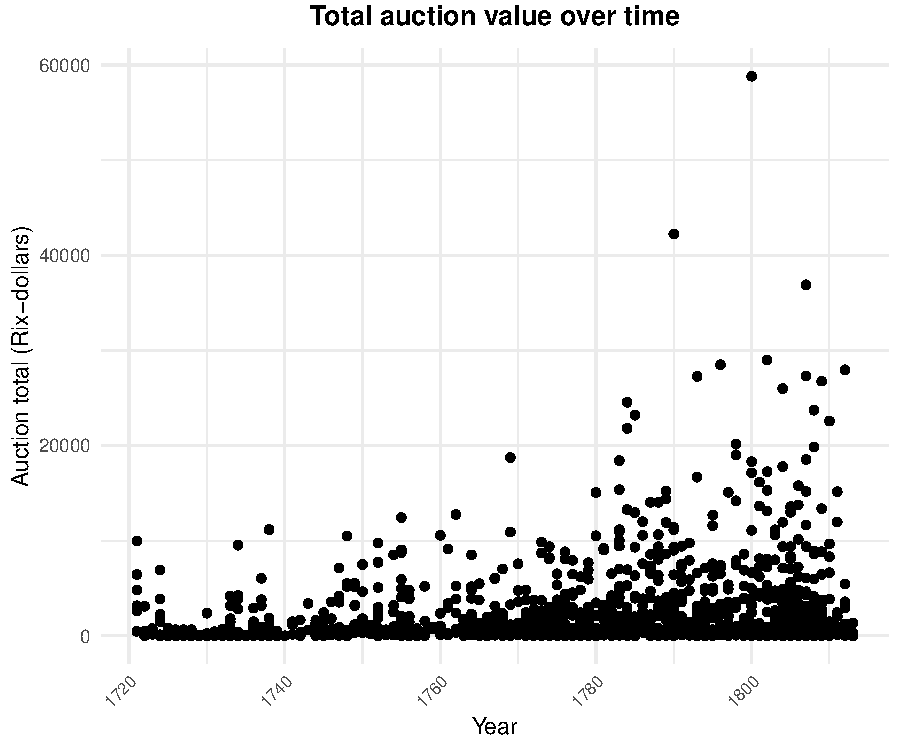
\includegraphics{Project_write_up_files/figure-latex/Figure1-1.pdf}

Figure 2 makes it clear that china, cups and chairs make up a large
amount of the household goods sold per auction. However, the number of
household goods, in absolute terms, does decline over time.

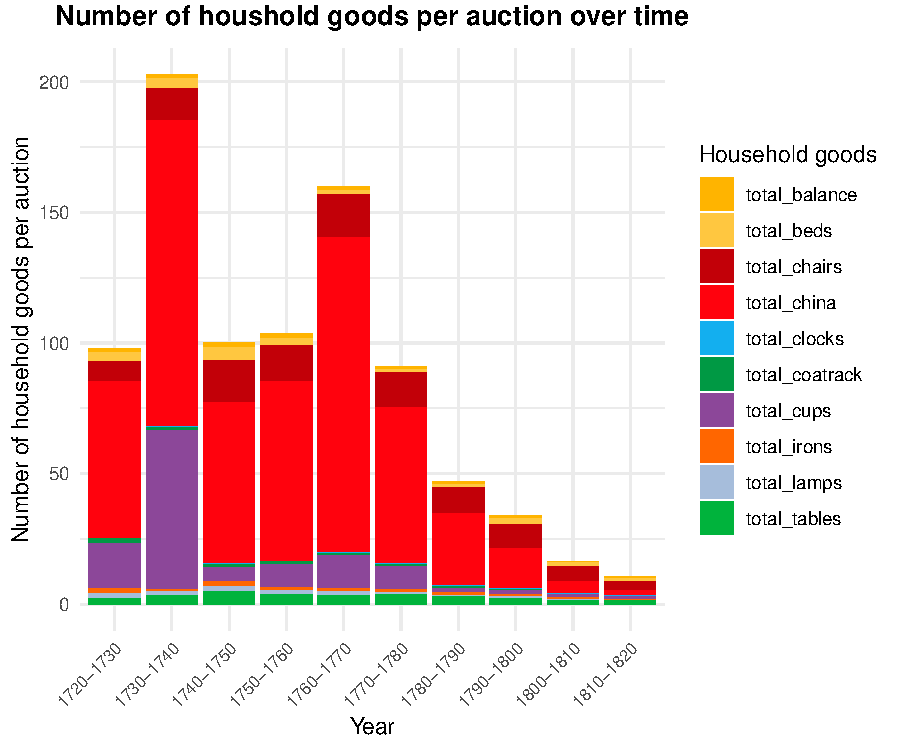
\includegraphics{Project_write_up_files/figure-latex/Figure2-1.pdf}

Figure 3 shows that utensils and plates make up the largest amount of
kitchen goods sold per auction. As with household goods, kitchen goods
also decline in absolute terms over time.

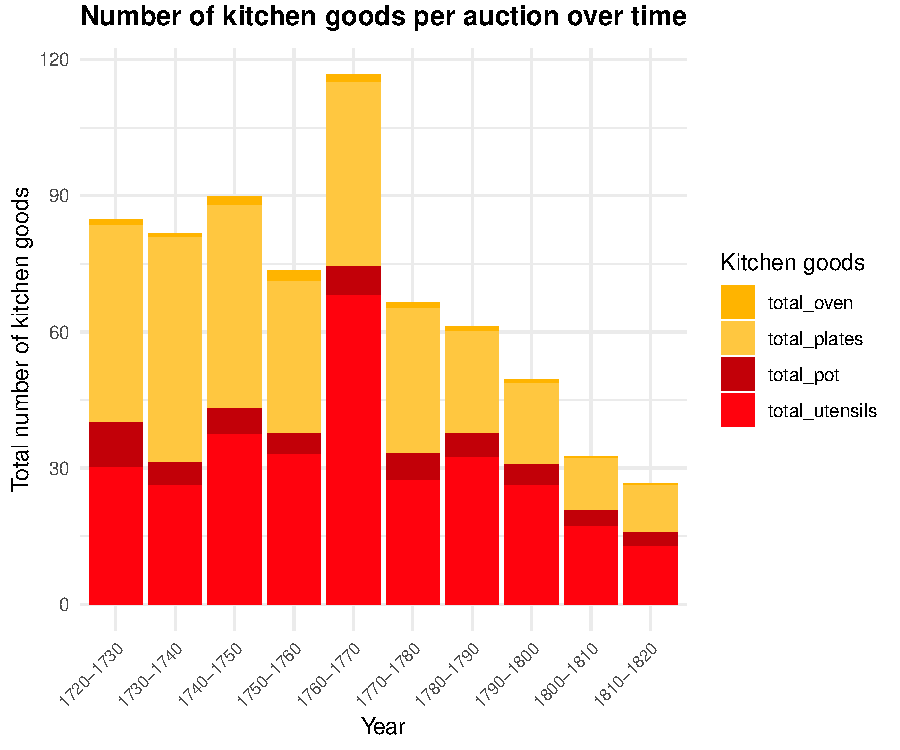
\includegraphics{Project_write_up_files/figure-latex/Figure3-1.pdf}

Figure 4 shows that the total number of farming goods is much higher
than that of household and kitchen goods which peak at 200 and 120,
respectively. Cattle and sheep are the most prominent farming goods sold
per auction.

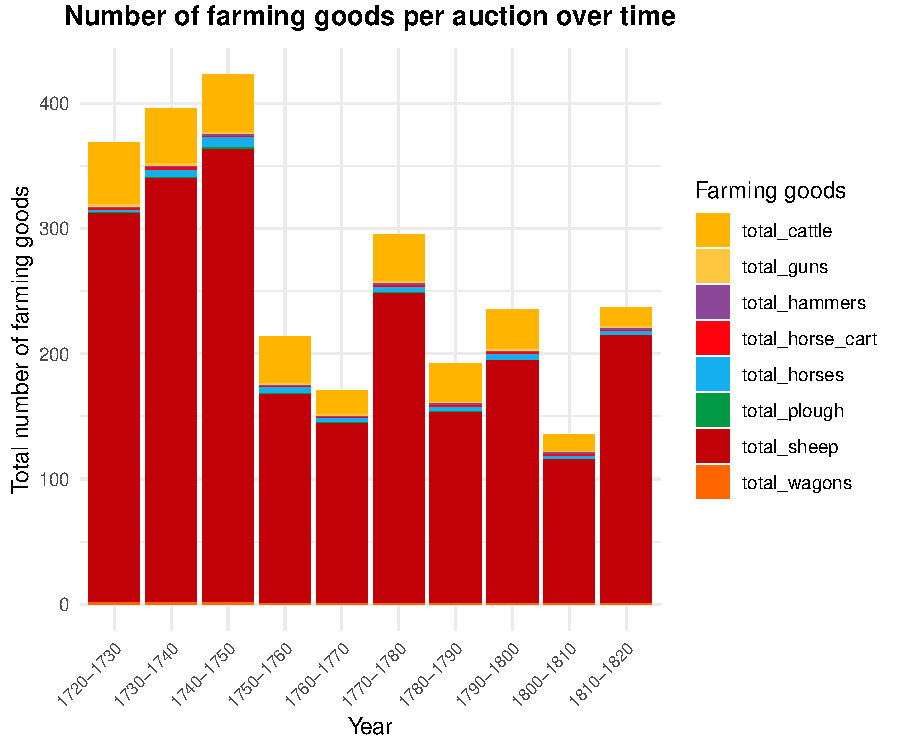
\includegraphics{Project_write_up_files/figure-latex/Figure4-1.pdf}

Figure 5 shows the average number of art products, books and slaves sold
per auction over time. The absolute number of select goods is lower than
the number of household, kitchen and farming goods.

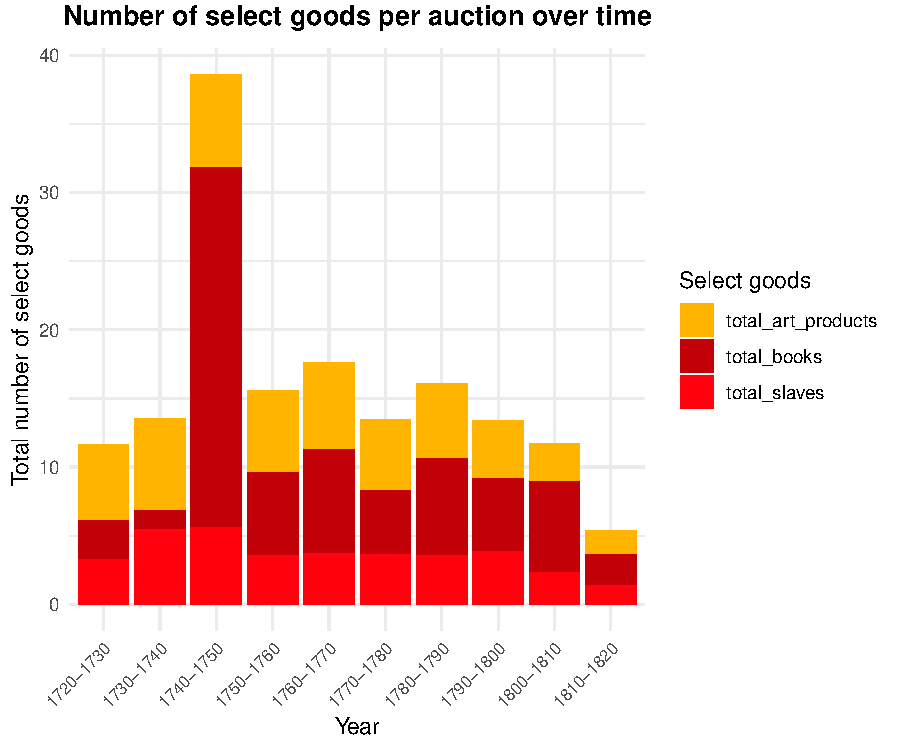
\includegraphics{Project_write_up_files/figure-latex/Figure5-1.pdf}

Figure 6 shows box plots of the number different types of goods that
were frequently purchased in auctions. For visuals purposes, the y-axis
was capped at 200 but there are a few outliers exceeding this number.
Cattle and utensils appear to be some of the most frequently purchased
goods throughout auctions yet the average number of goods per auction
for each type remains very low.

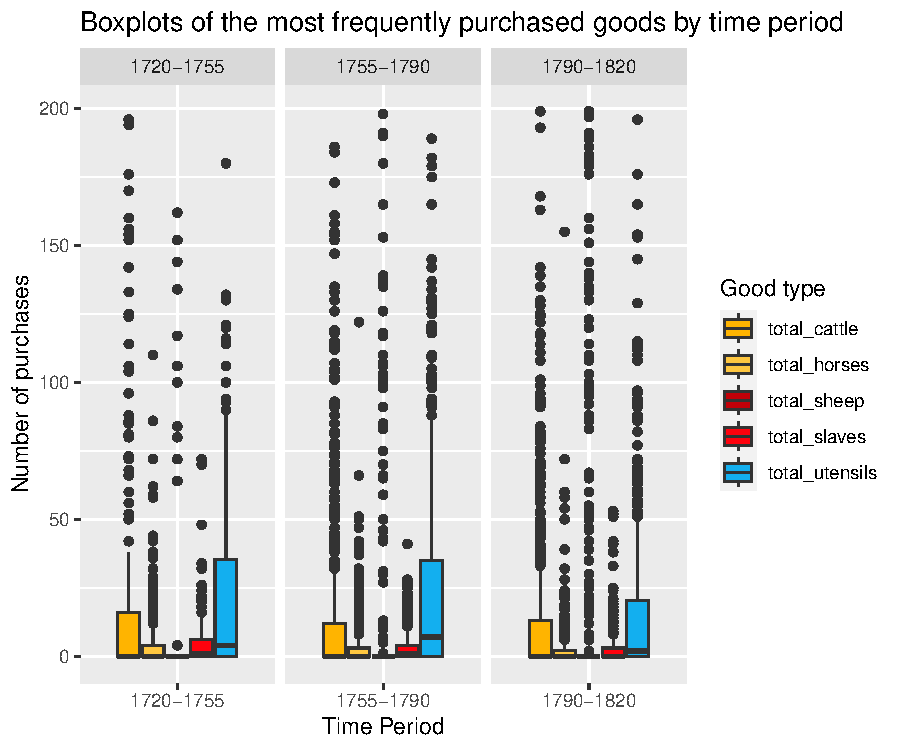
\includegraphics{Project_write_up_files/figure-latex/Figure6-1.pdf}

In terms of attendance by titled men and women, Figure 7 shows the
trends. There is a downward trend in attendance by titled purchasers
from 1750 and titled men always outnumber titled women at auctions.

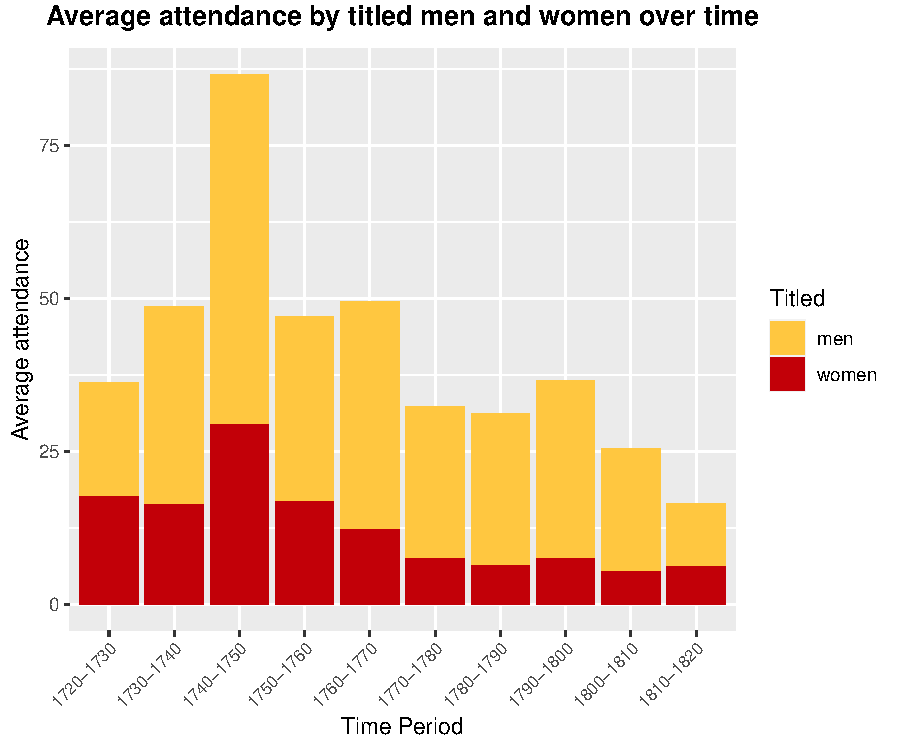
\includegraphics{Project_write_up_files/figure-latex/Figure7-1.pdf}

Figure 8 shows how certain good type purchases relate to total auction
values. This shows that the data is heavily clustered close to 0 due to
the small number of tagged goods present at each auction.

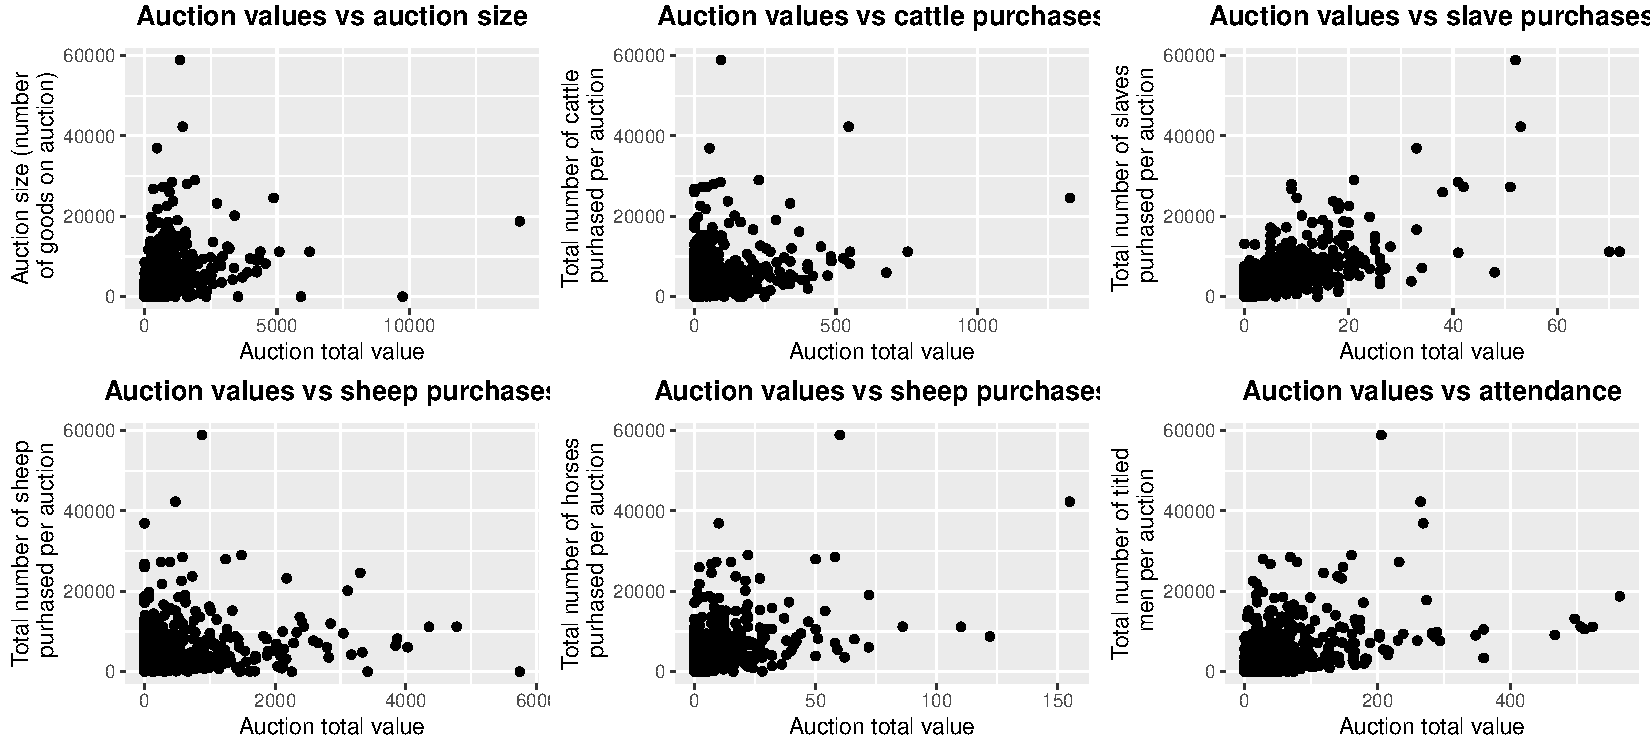
\includegraphics{Project_write_up_files/figure-latex/Figure8-1.pdf}

\hypertarget{target-and-feature-engineering}{%
\section*{Target and feature
engineering}\label{target-and-feature-engineering}}
\addcontentsline{toc}{section}{Target and feature engineering}

The target in this project is the auction total value. The features used
to predict the target include: the total number of items within a good
type per auction, total number of items within an auction (auction
size), number of titled men and women in attendance per auction and the
year of auction. Figure 9 provides evidence that the features are skewed
left. This is solved by applying a log transformation to all features
(except for the date).

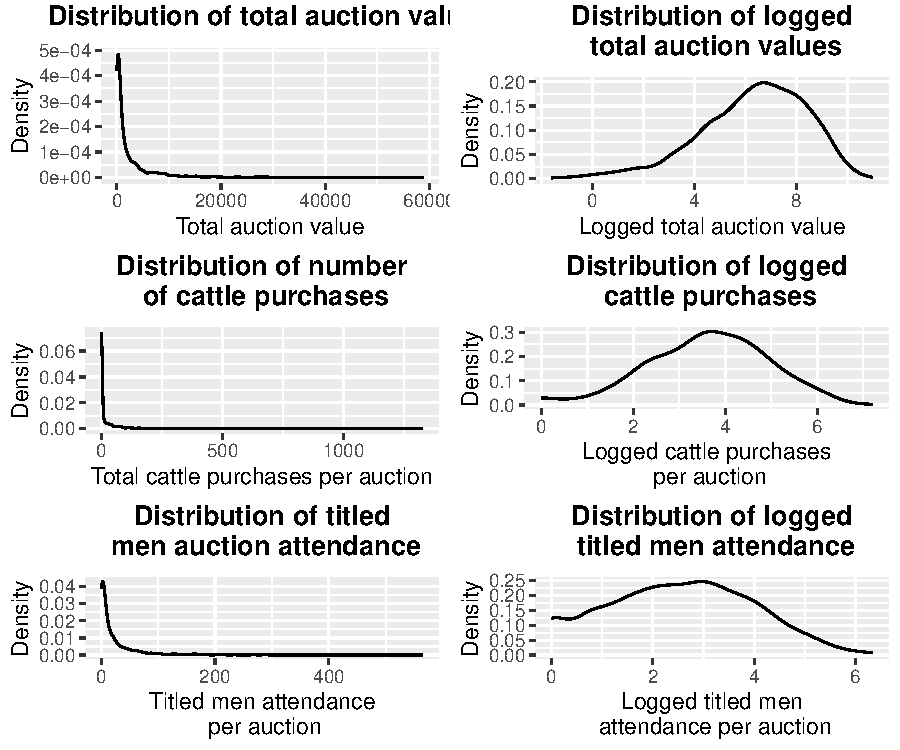
\includegraphics{Project_write_up_files/figure-latex/Figure9-1.pdf}

\begin{verbatim}
## TableGrob (3 x 2) "arrange": 6 grobs
##   z     cells    name           grob
## 1 1 (1-1,1-1) arrange gtable[layout]
## 2 2 (1-1,2-2) arrange gtable[layout]
## 3 3 (2-2,1-1) arrange gtable[layout]
## 4 4 (2-2,2-2) arrange gtable[layout]
## 5 5 (3-3,1-1) arrange gtable[layout]
## 6 6 (3-3,2-2) arrange gtable[layout]
\end{verbatim}

\hypertarget{methodology}{%
\section{Methodology}\label{methodology}}

This project aims to predict auction values based on different types of
goods present at an auction. Predicting a continuous, numerical value
presents a regression problem. As a result, the k-Nearest Neighbours
(KNN) model and a random forest model will be used. A linear regression
model will be used to determine how well machine learning models compare
to a regression. The metric used to assess the quality of the machine
learning predictions will be root-mean-squared-error (RMSE). This metric
indicates how far predictions are from actual values on average.
Additionally, r\^{}2 will be used to determine how well the model fits
the data. A default model will be run for each model before conducting
hyperparameter tuning to improve upon the model.

\hypertarget{knn-model}{%
\subsection{KNN model}\label{knn-model}}

The KNN model generates predictions for a new observation based on
matching it to the most similar training observations and aggregating
their values. When assessing a new observation (auction), it will
compare the bundle of goods present to other auctions with the most
similar bundles of goods sold and average their total values to
determine a prediction. Hyperperameter tuning is required to set the
optimal value of k. Figure 10 shows that k=5 is the optimal value. New
observations predictions will be the average of its five most similar
auctions.

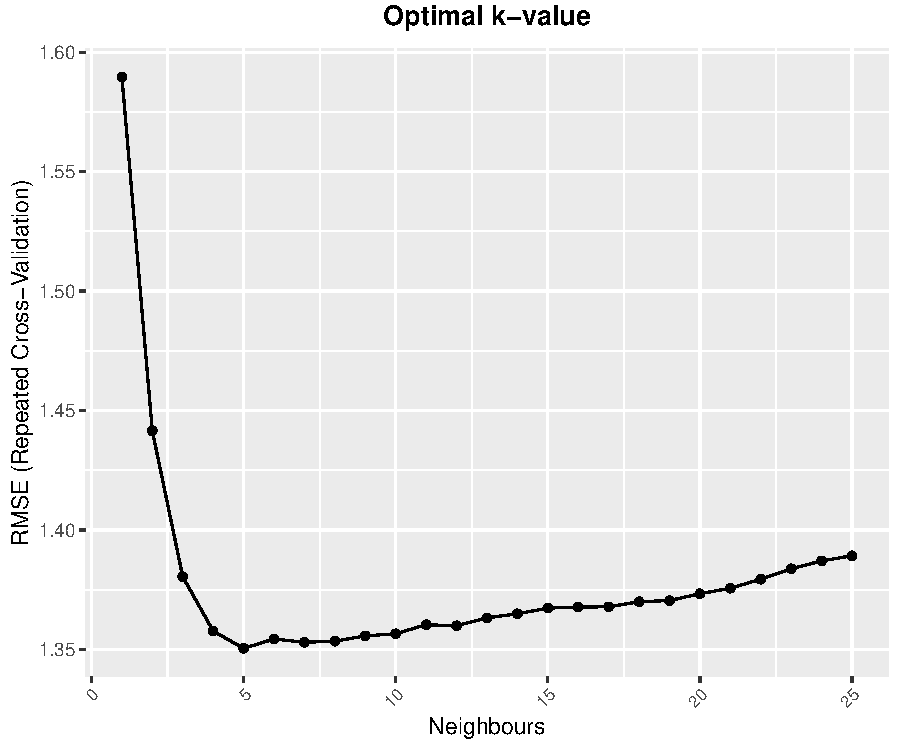
\includegraphics{Project_write_up_files/figure-latex/Figure10-1.pdf}

With the training data set, RMSE is 1.35 and r\^{}2 is 0.59. With the
testing data,however, RMSE reduces to 1.17 and r\^{}2 increases to 0.83.
This would indicate that the predictive accuracy and model fit improved
between the training and testing data. The mean logged auction total is
6.32 which means that predictions in the training set are on average
1.35 points off the actual auction value. Figure 11 shows that a very
small proportion of predictions are within 0.3 points of the actual
value. This indicates that knn is a poor model for predicting total
auction values. It is important to note that it is a problem that RMSE
decreases and r\^{}2 increases when moving from the training to the
testing dataset. One would expect to see the opposite. Possible reasons
for this may include data leakage. After checking for this, I could not
come to an explanation for why this was occuring.

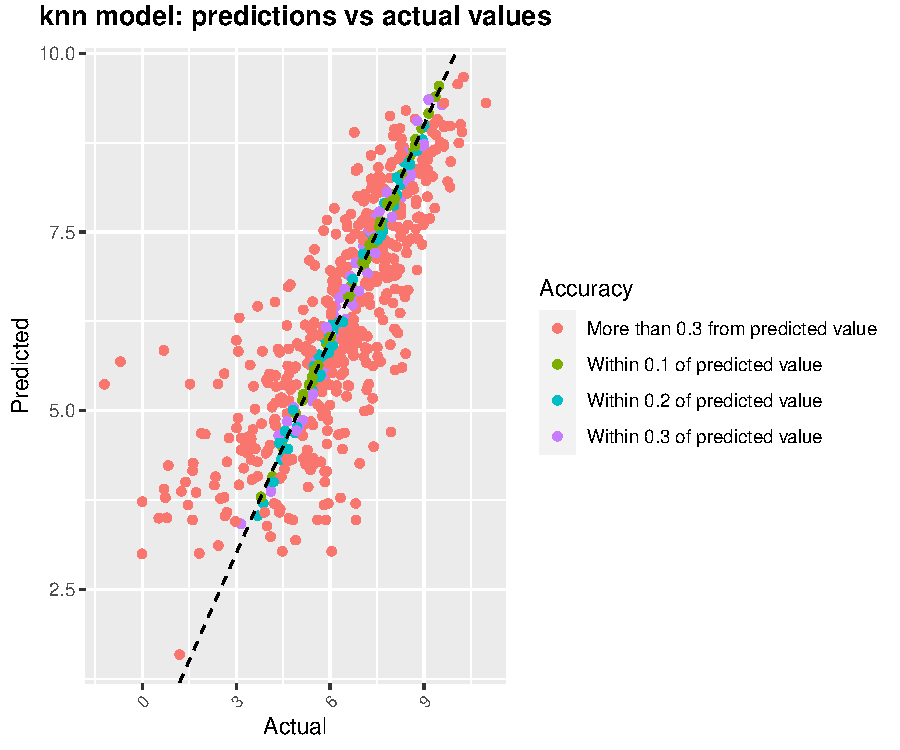
\includegraphics{Project_write_up_files/figure-latex/Fgiure11-1.pdf}

\hypertarget{random-forest-model}{%
\section{Random Forest Model}\label{random-forest-model}}

Random forest models include multiple decision trees to make
predictions. Decision trees are built independently on a subset of data
to introduce diversity among trees and reduce overfitting. Additionally,
random features are selected at each node of the tree to cover a wider
breadth of the data and include more robust predictions. Once the
decision trees are trained, predictions of each tree are aggregated to
generate predicitons. The randomness of random data and feature
selection decreases variance in predictions and aggregating tree-level
predictions minimises bias introduced at within trees. Tuning parameters
such as the number of trees within the random forest and the number of
features randomly selected at each node should improve predictions.
Furthermore, the node size can also be tuned as it refers to the minimum
number of observations required at a terminal node to ensure another
split.

The default model includes 500 trees, 10 features randomly selected at
each split and a target node size of 10. The RMSE is 1.1 and the r\^{}2
is 0.73. A random forest model offers information on each features'
importance in generating predictions. It is clear from Figure 12 that
the number of slaves at an auction is the most important feature,
followed by the size of the auction, the year the auction took place and
the number of titled men in attendance. These features make sense within
the context of the Cape Colony.

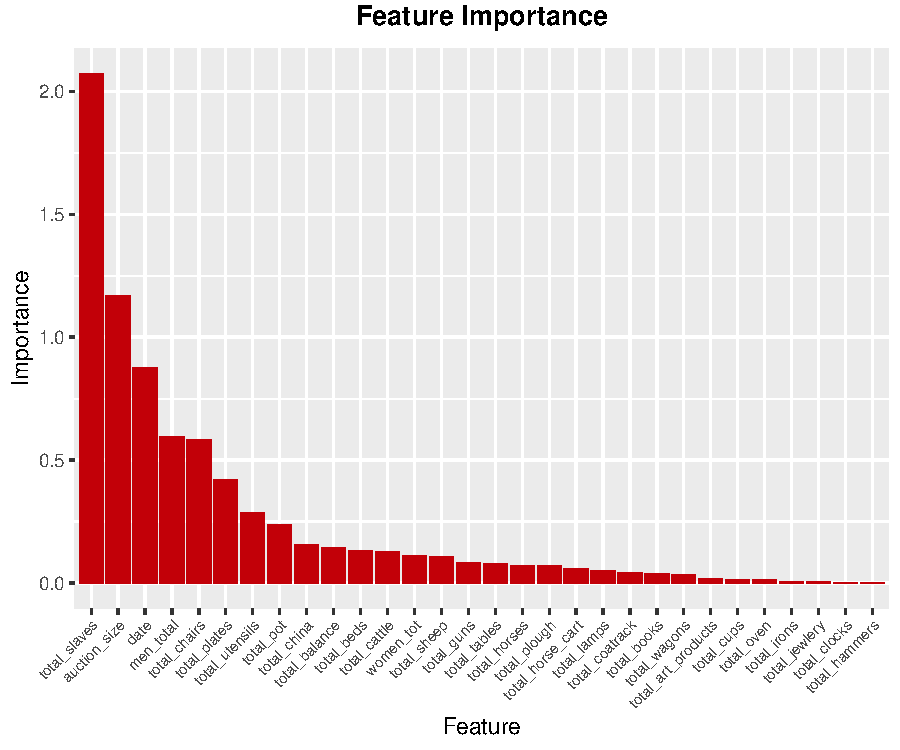
\includegraphics{Project_write_up_files/figure-latex/Figure12, -1.pdf}

After completing a grid search to tune parameters, the default model is
found to perform the best. When moving from the training to the testing
data, RMSE increases to 2.68. Figure 13 below shows that only a small
proportion of predictions are within 0.1 of the predicted value. Based
on RMSE scores, the knn model performs better than the random forest
model as its RMSE is 1.17.

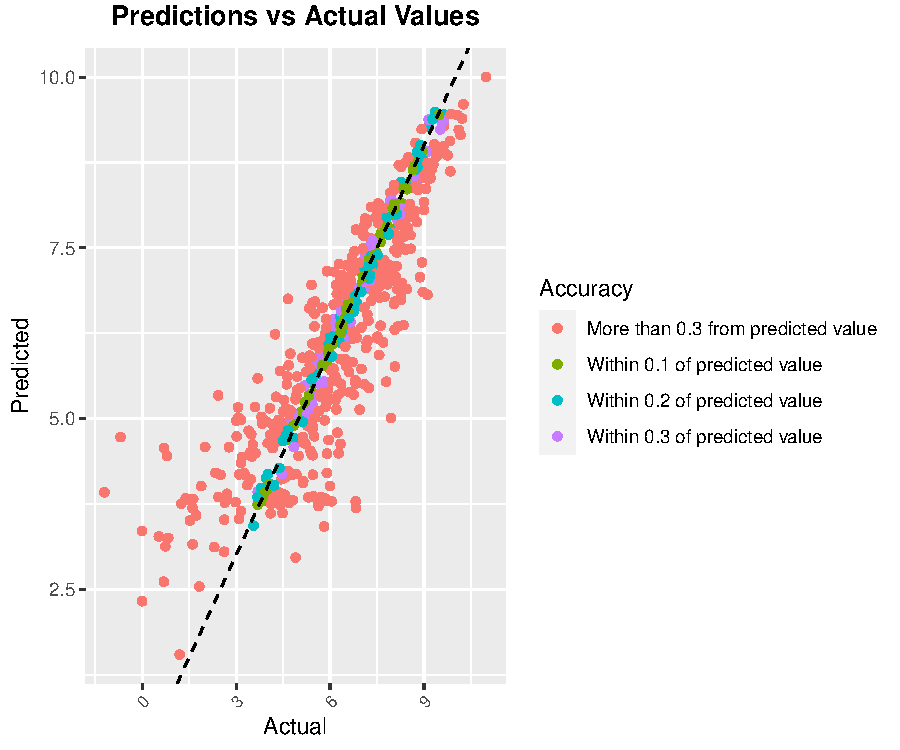
\includegraphics{Project_write_up_files/figure-latex/Figure13-1.pdf}

\hypertarget{linear-regression}{%
\section{Linear regression}\label{linear-regression}}

A linear regression is shown below. The RMSE is 1.13 and the r\^{}2 is
0.71. This linear regression model therefore performs than the machine
learning models with a higher prediction accuracy and better fit.

\begin{verbatim}
## 
## Call:
## lm(formula = auction_tot ~ ., data = ml_df)
## 
## Residuals:
##     Min      1Q  Median      3Q     Max 
## -6.5948 -0.5293  0.0539  0.6001  4.1455 
## 
## Coefficients:
##                     Estimate Std. Error t value Pr(>|t|)    
## (Intercept)        -0.313766   0.258401  -1.214 0.224846    
## total_beds          0.030920   0.051578   0.599 0.548949    
## total_books         0.015259   0.031399   0.486 0.627072    
## total_chairs        0.261487   0.050099   5.219 2.05e-07 ***
## total_china        -0.141661   0.030891  -4.586 4.91e-06 ***
## total_irons        -0.038633   0.080620  -0.479 0.631865    
## total_jewlery      -0.103175   0.084421  -1.222 0.221852    
## total_utensils      0.047291   0.029330   1.612 0.107102    
## total_art_products -0.033569   0.039911  -0.841 0.400440    
## total_balance      -0.117334   0.081773  -1.435 0.151540    
## total_clocks        0.035921   0.161785   0.222 0.824322    
## total_coatrack     -0.051524   0.084728  -0.608 0.543211    
## total_guns          0.131654   0.057684   2.282 0.022615 *  
## total_lamps        -0.102747   0.088199  -1.165 0.244232    
## total_oven          0.118811   0.066142   1.796 0.072653 .  
## total_plates        0.010087   0.040727   0.248 0.804424    
## total_pot          -0.143148   0.052739  -2.714 0.006721 ** 
## total_tables        0.027901   0.071554   0.390 0.696644    
## total_slaves        0.841320   0.046059  18.266  < 2e-16 ***
## total_cattle        0.118041   0.031233   3.779 0.000164 ***
## total_hammers       0.002032   0.070919   0.029 0.977149    
## total_horse_cart    0.061872   0.054133   1.143 0.253238    
## total_horses        0.026942   0.046512   0.579 0.562515    
## total_plough       -0.723920   0.107709  -6.721 2.58e-11 ***
## total_sheep         0.014712   0.024532   0.600 0.548800    
## total_wagons        0.108481   0.101793   1.066 0.286739    
## total_cups         -0.052726   0.035224  -1.497 0.134640    
## date                1.056096   0.057965  18.219  < 2e-16 ***
## auction_size        0.249047   0.033901   7.346 3.39e-13 ***
## women_tot           0.007093   0.033654   0.211 0.833102    
## men_total           0.205969   0.033692   6.113 1.25e-09 ***
## ---
## Signif. codes:  0 '***' 0.001 '**' 0.01 '*' 0.05 '.' 0.1 ' ' 1
## 
## Residual standard error: 1.138 on 1452 degrees of freedom
## Multiple R-squared:  0.705,  Adjusted R-squared:  0.6989 
## F-statistic: 115.7 on 30 and 1452 DF,  p-value: < 2.2e-16
\end{verbatim}

\begin{verbatim}
## [1] "\n\n```{=latex}\n \n  \\providecommand{\\huxb}[2]{\\arrayrulecolor[RGB]{#1}\\global\\arrayrulewidth=#2pt}\n  \\providecommand{\\huxvb}[2]{\\color[RGB]{#1}\\vrule width #2pt}\n  \\providecommand{\\huxtpad}[1]{\\rule{0pt}{#1}}\n  \\providecommand{\\huxbpad}[1]{\\rule[-#1]{0pt}{#1}}\n\n\\begin{table}[ht]\n\\begin{centerbox}\n\\begin{threeparttable}\n\\captionsetup{justification=centering,singlelinecheck=off}\n\\caption{Auction total value regression}\n \\label{tab:unnamed-chunk-1}\n\\setlength{\\tabcolsep}{0pt}\n\\begin{tabular}{l l}\n\n\n\\hhline{>{\\huxb{255, 255, 255}{0.4}}->{\\huxb{0, 0, 0}{0.4}}-}\n\\arrayrulecolor{black}\n\n\\multicolumn{1}{!{\\huxvb{0, 0, 0}{0}}l!{\\huxvb{0, 0, 0}{0}}}{\\huxtpad{6pt + 1em}\\raggedright \\hspace{6pt} (Intercept) \\hspace{6pt}\\huxbpad{6pt}} &\n\\multicolumn{1}{r!{\\huxvb{0, 0, 0}{0}}}{\\huxtpad{6pt + 1em}\\raggedleft \\hspace{6pt} -0.314\\hphantom{0}\\hphantom{0}\\hphantom{0}\\hphantom{0} \\hspace{6pt}\\huxbpad{6pt}} \\tabularnewline[-0.5pt]\n\n\n\\hhline{}\n\\arrayrulecolor{black}\n\n\\multicolumn{1}{!{\\huxvb{0, 0, 0}{0}}l!{\\huxvb{0, 0, 0}{0}}}{\\huxtpad{6pt + 1em}\\raggedright \\hspace{6pt}  \\hspace{6pt}\\huxbpad{6pt}} &\n\\multicolumn{1}{r!{\\huxvb{0, 0, 0}{0}}}{\\huxtpad{6pt + 1em}\\raggedleft \\hspace{6pt} (0.258)\\hphantom{0}\\hphantom{0}\\hphantom{0} \\hspace{6pt}\\huxbpad{6pt}} \\tabularnewline[-0.5pt]\n\n\n\\hhline{}\n\\arrayrulecolor{black}\n\n\\multicolumn{1}{!{\\huxvb{0, 0, 0}{0}}l!{\\huxvb{0, 0, 0}{0}}}{\\huxtpad{6pt + 1em}\\raggedright \\hspace{6pt} total\\_beds \\hspace{6pt}\\huxbpad{6pt}} &\n\\multicolumn{1}{r!{\\huxvb{0, 0, 0}{0}}}{\\huxtpad{6pt + 1em}\\raggedleft \\hspace{6pt} 0.031\\hphantom{0}\\hphantom{0}\\hphantom{0}\\hphantom{0} \\hspace{6pt}\\huxbpad{6pt}} \\tabularnewline[-0.5pt]\n\n\n\\hhline{}\n\\arrayrulecolor{black}\n\n\\multicolumn{1}{!{\\huxvb{0, 0, 0}{0}}l!{\\huxvb{0, 0, 0}{0}}}{\\huxtpad{6pt + 1em}\\raggedright \\hspace{6pt}  \\hspace{6pt}\\huxbpad{6pt}} &\n\\multicolumn{1}{r!{\\huxvb{0, 0, 0}{0}}}{\\huxtpad{6pt + 1em}\\raggedleft \\hspace{6pt} (0.052)\\hphantom{0}\\hphantom{0}\\hphantom{0} \\hspace{6pt}\\huxbpad{6pt}} \\tabularnewline[-0.5pt]\n\n\n\\hhline{}\n\\arrayrulecolor{black}\n\n\\multicolumn{1}{!{\\huxvb{0, 0, 0}{0}}l!{\\huxvb{0, 0, 0}{0}}}{\\huxtpad{6pt + 1em}\\raggedright \\hspace{6pt} total\\_books \\hspace{6pt}\\huxbpad{6pt}} &\n\\multicolumn{1}{r!{\\huxvb{0, 0, 0}{0}}}{\\huxtpad{6pt + 1em}\\raggedleft \\hspace{6pt} 0.015\\hphantom{0}\\hphantom{0}\\hphantom{0}\\hphantom{0} \\hspace{6pt}\\huxbpad{6pt}} \\tabularnewline[-0.5pt]\n\n\n\\hhline{}\n\\arrayrulecolor{black}\n\n\\multicolumn{1}{!{\\huxvb{0, 0, 0}{0}}l!{\\huxvb{0, 0, 0}{0}}}{\\huxtpad{6pt + 1em}\\raggedright \\hspace{6pt}  \\hspace{6pt}\\huxbpad{6pt}} &\n\\multicolumn{1}{r!{\\huxvb{0, 0, 0}{0}}}{\\huxtpad{6pt + 1em}\\raggedleft \\hspace{6pt} (0.031)\\hphantom{0}\\hphantom{0}\\hphantom{0} \\hspace{6pt}\\huxbpad{6pt}} \\tabularnewline[-0.5pt]\n\n\n\\hhline{}\n\\arrayrulecolor{black}\n\n\\multicolumn{1}{!{\\huxvb{0, 0, 0}{0}}l!{\\huxvb{0, 0, 0}{0}}}{\\huxtpad{6pt + 1em}\\raggedright \\hspace{6pt} total\\_chairs \\hspace{6pt}\\huxbpad{6pt}} &\n\\multicolumn{1}{r!{\\huxvb{0, 0, 0}{0}}}{\\huxtpad{6pt + 1em}\\raggedleft \\hspace{6pt} 0.261 *** \\hspace{6pt}\\huxbpad{6pt}} \\tabularnewline[-0.5pt]\n\n\n\\hhline{}\n\\arrayrulecolor{black}\n\n\\multicolumn{1}{!{\\huxvb{0, 0, 0}{0}}l!{\\huxvb{0, 0, 0}{0}}}{\\huxtpad{6pt + 1em}\\raggedright \\hspace{6pt}  \\hspace{6pt}\\huxbpad{6pt}} &\n\\multicolumn{1}{r!{\\huxvb{0, 0, 0}{0}}}{\\huxtpad{6pt + 1em}\\raggedleft \\hspace{6pt} (0.050)\\hphantom{0}\\hphantom{0}\\hphantom{0} \\hspace{6pt}\\huxbpad{6pt}} \\tabularnewline[-0.5pt]\n\n\n\\hhline{}\n\\arrayrulecolor{black}\n\n\\multicolumn{1}{!{\\huxvb{0, 0, 0}{0}}l!{\\huxvb{0, 0, 0}{0}}}{\\huxtpad{6pt + 1em}\\raggedright \\hspace{6pt} total\\_china \\hspace{6pt}\\huxbpad{6pt}} &\n\\multicolumn{1}{r!{\\huxvb{0, 0, 0}{0}}}{\\huxtpad{6pt + 1em}\\raggedleft \\hspace{6pt} -0.142 *** \\hspace{6pt}\\huxbpad{6pt}} \\tabularnewline[-0.5pt]\n\n\n\\hhline{}\n\\arrayrulecolor{black}\n\n\\multicolumn{1}{!{\\huxvb{0, 0, 0}{0}}l!{\\huxvb{0, 0, 0}{0}}}{\\huxtpad{6pt + 1em}\\raggedright \\hspace{6pt}  \\hspace{6pt}\\huxbpad{6pt}} &\n\\multicolumn{1}{r!{\\huxvb{0, 0, 0}{0}}}{\\huxtpad{6pt + 1em}\\raggedleft \\hspace{6pt} (0.031)\\hphantom{0}\\hphantom{0}\\hphantom{0} \\hspace{6pt}\\huxbpad{6pt}} \\tabularnewline[-0.5pt]\n\n\n\\hhline{}\n\\arrayrulecolor{black}\n\n\\multicolumn{1}{!{\\huxvb{0, 0, 0}{0}}l!{\\huxvb{0, 0, 0}{0}}}{\\huxtpad{6pt + 1em}\\raggedright \\hspace{6pt} total\\_irons \\hspace{6pt}\\huxbpad{6pt}} &\n\\multicolumn{1}{r!{\\huxvb{0, 0, 0}{0}}}{\\huxtpad{6pt + 1em}\\raggedleft \\hspace{6pt} -0.039\\hphantom{0}\\hphantom{0}\\hphantom{0}\\hphantom{0} \\hspace{6pt}\\huxbpad{6pt}} \\tabularnewline[-0.5pt]\n\n\n\\hhline{}\n\\arrayrulecolor{black}\n\n\\multicolumn{1}{!{\\huxvb{0, 0, 0}{0}}l!{\\huxvb{0, 0, 0}{0}}}{\\huxtpad{6pt + 1em}\\raggedright \\hspace{6pt}  \\hspace{6pt}\\huxbpad{6pt}} &\n\\multicolumn{1}{r!{\\huxvb{0, 0, 0}{0}}}{\\huxtpad{6pt + 1em}\\raggedleft \\hspace{6pt} (0.081)\\hphantom{0}\\hphantom{0}\\hphantom{0} \\hspace{6pt}\\huxbpad{6pt}} \\tabularnewline[-0.5pt]\n\n\n\\hhline{}\n\\arrayrulecolor{black}\n\n\\multicolumn{1}{!{\\huxvb{0, 0, 0}{0}}l!{\\huxvb{0, 0, 0}{0}}}{\\huxtpad{6pt + 1em}\\raggedright \\hspace{6pt} total\\_jewlery \\hspace{6pt}\\huxbpad{6pt}} &\n\\multicolumn{1}{r!{\\huxvb{0, 0, 0}{0}}}{\\huxtpad{6pt + 1em}\\raggedleft \\hspace{6pt} -0.103\\hphantom{0}\\hphantom{0}\\hphantom{0}\\hphantom{0} \\hspace{6pt}\\huxbpad{6pt}} \\tabularnewline[-0.5pt]\n\n\n\\hhline{}\n\\arrayrulecolor{black}\n\n\\multicolumn{1}{!{\\huxvb{0, 0, 0}{0}}l!{\\huxvb{0, 0, 0}{0}}}{\\huxtpad{6pt + 1em}\\raggedright \\hspace{6pt}  \\hspace{6pt}\\huxbpad{6pt}} &\n\\multicolumn{1}{r!{\\huxvb{0, 0, 0}{0}}}{\\huxtpad{6pt + 1em}\\raggedleft \\hspace{6pt} (0.084)\\hphantom{0}\\hphantom{0}\\hphantom{0} \\hspace{6pt}\\huxbpad{6pt}} \\tabularnewline[-0.5pt]\n\n\n\\hhline{}\n\\arrayrulecolor{black}\n\n\\multicolumn{1}{!{\\huxvb{0, 0, 0}{0}}l!{\\huxvb{0, 0, 0}{0}}}{\\huxtpad{6pt + 1em}\\raggedright \\hspace{6pt} total\\_utensils \\hspace{6pt}\\huxbpad{6pt}} &\n\\multicolumn{1}{r!{\\huxvb{0, 0, 0}{0}}}{\\huxtpad{6pt + 1em}\\raggedleft \\hspace{6pt} 0.047\\hphantom{0}\\hphantom{0}\\hphantom{0}\\hphantom{0} \\hspace{6pt}\\huxbpad{6pt}} \\tabularnewline[-0.5pt]\n\n\n\\hhline{}\n\\arrayrulecolor{black}\n\n\\multicolumn{1}{!{\\huxvb{0, 0, 0}{0}}l!{\\huxvb{0, 0, 0}{0}}}{\\huxtpad{6pt + 1em}\\raggedright \\hspace{6pt}  \\hspace{6pt}\\huxbpad{6pt}} &\n\\multicolumn{1}{r!{\\huxvb{0, 0, 0}{0}}}{\\huxtpad{6pt + 1em}\\raggedleft \\hspace{6pt} (0.029)\\hphantom{0}\\hphantom{0}\\hphantom{0} \\hspace{6pt}\\huxbpad{6pt}} \\tabularnewline[-0.5pt]\n\n\n\\hhline{}\n\\arrayrulecolor{black}\n\n\\multicolumn{1}{!{\\huxvb{0, 0, 0}{0}}l!{\\huxvb{0, 0, 0}{0}}}{\\huxtpad{6pt + 1em}\\raggedright \\hspace{6pt} total\\_art\\_products \\hspace{6pt}\\huxbpad{6pt}} &\n\\multicolumn{1}{r!{\\huxvb{0, 0, 0}{0}}}{\\huxtpad{6pt + 1em}\\raggedleft \\hspace{6pt} -0.034\\hphantom{0}\\hphantom{0}\\hphantom{0}\\hphantom{0} \\hspace{6pt}\\huxbpad{6pt}} \\tabularnewline[-0.5pt]\n\n\n\\hhline{}\n\\arrayrulecolor{black}\n\n\\multicolumn{1}{!{\\huxvb{0, 0, 0}{0}}l!{\\huxvb{0, 0, 0}{0}}}{\\huxtpad{6pt + 1em}\\raggedright \\hspace{6pt}  \\hspace{6pt}\\huxbpad{6pt}} &\n\\multicolumn{1}{r!{\\huxvb{0, 0, 0}{0}}}{\\huxtpad{6pt + 1em}\\raggedleft \\hspace{6pt} (0.040)\\hphantom{0}\\hphantom{0}\\hphantom{0} \\hspace{6pt}\\huxbpad{6pt}} \\tabularnewline[-0.5pt]\n\n\n\\hhline{}\n\\arrayrulecolor{black}\n\n\\multicolumn{1}{!{\\huxvb{0, 0, 0}{0}}l!{\\huxvb{0, 0, 0}{0}}}{\\huxtpad{6pt + 1em}\\raggedright \\hspace{6pt} total\\_balance \\hspace{6pt}\\huxbpad{6pt}} &\n\\multicolumn{1}{r!{\\huxvb{0, 0, 0}{0}}}{\\huxtpad{6pt + 1em}\\raggedleft \\hspace{6pt} -0.117\\hphantom{0}\\hphantom{0}\\hphantom{0}\\hphantom{0} \\hspace{6pt}\\huxbpad{6pt}} \\tabularnewline[-0.5pt]\n\n\n\\hhline{}\n\\arrayrulecolor{black}\n\n\\multicolumn{1}{!{\\huxvb{0, 0, 0}{0}}l!{\\huxvb{0, 0, 0}{0}}}{\\huxtpad{6pt + 1em}\\raggedright \\hspace{6pt}  \\hspace{6pt}\\huxbpad{6pt}} &\n\\multicolumn{1}{r!{\\huxvb{0, 0, 0}{0}}}{\\huxtpad{6pt + 1em}\\raggedleft \\hspace{6pt} (0.082)\\hphantom{0}\\hphantom{0}\\hphantom{0} \\hspace{6pt}\\huxbpad{6pt}} \\tabularnewline[-0.5pt]\n\n\n\\hhline{}\n\\arrayrulecolor{black}\n\n\\multicolumn{1}{!{\\huxvb{0, 0, 0}{0}}l!{\\huxvb{0, 0, 0}{0}}}{\\huxtpad{6pt + 1em}\\raggedright \\hspace{6pt} total\\_clocks \\hspace{6pt}\\huxbpad{6pt}} &\n\\multicolumn{1}{r!{\\huxvb{0, 0, 0}{0}}}{\\huxtpad{6pt + 1em}\\raggedleft \\hspace{6pt} 0.036\\hphantom{0}\\hphantom{0}\\hphantom{0}\\hphantom{0} \\hspace{6pt}\\huxbpad{6pt}} \\tabularnewline[-0.5pt]\n\n\n\\hhline{}\n\\arrayrulecolor{black}\n\n\\multicolumn{1}{!{\\huxvb{0, 0, 0}{0}}l!{\\huxvb{0, 0, 0}{0}}}{\\huxtpad{6pt + 1em}\\raggedright \\hspace{6pt}  \\hspace{6pt}\\huxbpad{6pt}} &\n\\multicolumn{1}{r!{\\huxvb{0, 0, 0}{0}}}{\\huxtpad{6pt + 1em}\\raggedleft \\hspace{6pt} (0.162)\\hphantom{0}\\hphantom{0}\\hphantom{0} \\hspace{6pt}\\huxbpad{6pt}} \\tabularnewline[-0.5pt]\n\n\n\\hhline{}\n\\arrayrulecolor{black}\n\n\\multicolumn{1}{!{\\huxvb{0, 0, 0}{0}}l!{\\huxvb{0, 0, 0}{0}}}{\\huxtpad{6pt + 1em}\\raggedright \\hspace{6pt} total\\_coatrack \\hspace{6pt}\\huxbpad{6pt}} &\n\\multicolumn{1}{r!{\\huxvb{0, 0, 0}{0}}}{\\huxtpad{6pt + 1em}\\raggedleft \\hspace{6pt} -0.052\\hphantom{0}\\hphantom{0}\\hphantom{0}\\hphantom{0} \\hspace{6pt}\\huxbpad{6pt}} \\tabularnewline[-0.5pt]\n\n\n\\hhline{}\n\\arrayrulecolor{black}\n\n\\multicolumn{1}{!{\\huxvb{0, 0, 0}{0}}l!{\\huxvb{0, 0, 0}{0}}}{\\huxtpad{6pt + 1em}\\raggedright \\hspace{6pt}  \\hspace{6pt}\\huxbpad{6pt}} &\n\\multicolumn{1}{r!{\\huxvb{0, 0, 0}{0}}}{\\huxtpad{6pt + 1em}\\raggedleft \\hspace{6pt} (0.085)\\hphantom{0}\\hphantom{0}\\hphantom{0} \\hspace{6pt}\\huxbpad{6pt}} \\tabularnewline[-0.5pt]\n\n\n\\hhline{}\n\\arrayrulecolor{black}\n\n\\multicolumn{1}{!{\\huxvb{0, 0, 0}{0}}l!{\\huxvb{0, 0, 0}{0}}}{\\huxtpad{6pt + 1em}\\raggedright \\hspace{6pt} total\\_guns \\hspace{6pt}\\huxbpad{6pt}} &\n\\multicolumn{1}{r!{\\huxvb{0, 0, 0}{0}}}{\\huxtpad{6pt + 1em}\\raggedleft \\hspace{6pt} 0.132 *\\hphantom{0}\\hphantom{0} \\hspace{6pt}\\huxbpad{6pt}} \\tabularnewline[-0.5pt]\n\n\n\\hhline{}\n\\arrayrulecolor{black}\n\n\\multicolumn{1}{!{\\huxvb{0, 0, 0}{0}}l!{\\huxvb{0, 0, 0}{0}}}{\\huxtpad{6pt + 1em}\\raggedright \\hspace{6pt}  \\hspace{6pt}\\huxbpad{6pt}} &\n\\multicolumn{1}{r!{\\huxvb{0, 0, 0}{0}}}{\\huxtpad{6pt + 1em}\\raggedleft \\hspace{6pt} (0.058)\\hphantom{0}\\hphantom{0}\\hphantom{0} \\hspace{6pt}\\huxbpad{6pt}} \\tabularnewline[-0.5pt]\n\n\n\\hhline{}\n\\arrayrulecolor{black}\n\n\\multicolumn{1}{!{\\huxvb{0, 0, 0}{0}}l!{\\huxvb{0, 0, 0}{0}}}{\\huxtpad{6pt + 1em}\\raggedright \\hspace{6pt} total\\_lamps \\hspace{6pt}\\huxbpad{6pt}} &\n\\multicolumn{1}{r!{\\huxvb{0, 0, 0}{0}}}{\\huxtpad{6pt + 1em}\\raggedleft \\hspace{6pt} -0.103\\hphantom{0}\\hphantom{0}\\hphantom{0}\\hphantom{0} \\hspace{6pt}\\huxbpad{6pt}} \\tabularnewline[-0.5pt]\n\n\n\\hhline{}\n\\arrayrulecolor{black}\n\n\\multicolumn{1}{!{\\huxvb{0, 0, 0}{0}}l!{\\huxvb{0, 0, 0}{0}}}{\\huxtpad{6pt + 1em}\\raggedright \\hspace{6pt}  \\hspace{6pt}\\huxbpad{6pt}} &\n\\multicolumn{1}{r!{\\huxvb{0, 0, 0}{0}}}{\\huxtpad{6pt + 1em}\\raggedleft \\hspace{6pt} (0.088)\\hphantom{0}\\hphantom{0}\\hphantom{0} \\hspace{6pt}\\huxbpad{6pt}} \\tabularnewline[-0.5pt]\n\n\n\\hhline{}\n\\arrayrulecolor{black}\n\n\\multicolumn{1}{!{\\huxvb{0, 0, 0}{0}}l!{\\huxvb{0, 0, 0}{0}}}{\\huxtpad{6pt + 1em}\\raggedright \\hspace{6pt} total\\_oven \\hspace{6pt}\\huxbpad{6pt}} &\n\\multicolumn{1}{r!{\\huxvb{0, 0, 0}{0}}}{\\huxtpad{6pt + 1em}\\raggedleft \\hspace{6pt} 0.119\\hphantom{0}\\hphantom{0}\\hphantom{0}\\hphantom{0} \\hspace{6pt}\\huxbpad{6pt}} \\tabularnewline[-0.5pt]\n\n\n\\hhline{}\n\\arrayrulecolor{black}\n\n\\multicolumn{1}{!{\\huxvb{0, 0, 0}{0}}l!{\\huxvb{0, 0, 0}{0}}}{\\huxtpad{6pt + 1em}\\raggedright \\hspace{6pt}  \\hspace{6pt}\\huxbpad{6pt}} &\n\\multicolumn{1}{r!{\\huxvb{0, 0, 0}{0}}}{\\huxtpad{6pt + 1em}\\raggedleft \\hspace{6pt} (0.066)\\hphantom{0}\\hphantom{0}\\hphantom{0} \\hspace{6pt}\\huxbpad{6pt}} \\tabularnewline[-0.5pt]\n\n\n\\hhline{}\n\\arrayrulecolor{black}\n\n\\multicolumn{1}{!{\\huxvb{0, 0, 0}{0}}l!{\\huxvb{0, 0, 0}{0}}}{\\huxtpad{6pt + 1em}\\raggedright \\hspace{6pt} total\\_plates \\hspace{6pt}\\huxbpad{6pt}} &\n\\multicolumn{1}{r!{\\huxvb{0, 0, 0}{0}}}{\\huxtpad{6pt + 1em}\\raggedleft \\hspace{6pt} 0.010\\hphantom{0}\\hphantom{0}\\hphantom{0}\\hphantom{0} \\hspace{6pt}\\huxbpad{6pt}} \\tabularnewline[-0.5pt]\n\n\n\\hhline{}\n\\arrayrulecolor{black}\n\n\\multicolumn{1}{!{\\huxvb{0, 0, 0}{0}}l!{\\huxvb{0, 0, 0}{0}}}{\\huxtpad{6pt + 1em}\\raggedright \\hspace{6pt}  \\hspace{6pt}\\huxbpad{6pt}} &\n\\multicolumn{1}{r!{\\huxvb{0, 0, 0}{0}}}{\\huxtpad{6pt + 1em}\\raggedleft \\hspace{6pt} (0.041)\\hphantom{0}\\hphantom{0}\\hphantom{0} \\hspace{6pt}\\huxbpad{6pt}} \\tabularnewline[-0.5pt]\n\n\n\\hhline{}\n\\arrayrulecolor{black}\n\n\\multicolumn{1}{!{\\huxvb{0, 0, 0}{0}}l!{\\huxvb{0, 0, 0}{0}}}{\\huxtpad{6pt + 1em}\\raggedright \\hspace{6pt} total\\_pot \\hspace{6pt}\\huxbpad{6pt}} &\n\\multicolumn{1}{r!{\\huxvb{0, 0, 0}{0}}}{\\huxtpad{6pt + 1em}\\raggedleft \\hspace{6pt} -0.143 **\\hphantom{0} \\hspace{6pt}\\huxbpad{6pt}} \\tabularnewline[-0.5pt]\n\n\n\\hhline{}\n\\arrayrulecolor{black}\n\n\\multicolumn{1}{!{\\huxvb{0, 0, 0}{0}}l!{\\huxvb{0, 0, 0}{0}}}{\\huxtpad{6pt + 1em}\\raggedright \\hspace{6pt}  \\hspace{6pt}\\huxbpad{6pt}} &\n\\multicolumn{1}{r!{\\huxvb{0, 0, 0}{0}}}{\\huxtpad{6pt + 1em}\\raggedleft \\hspace{6pt} (0.053)\\hphantom{0}\\hphantom{0}\\hphantom{0} \\hspace{6pt}\\huxbpad{6pt}} \\tabularnewline[-0.5pt]\n\n\n\\hhline{}\n\\arrayrulecolor{black}\n\n\\multicolumn{1}{!{\\huxvb{0, 0, 0}{0}}l!{\\huxvb{0, 0, 0}{0}}}{\\huxtpad{6pt + 1em}\\raggedright \\hspace{6pt} total\\_tables \\hspace{6pt}\\huxbpad{6pt}} &\n\\multicolumn{1}{r!{\\huxvb{0, 0, 0}{0}}}{\\huxtpad{6pt + 1em}\\raggedleft \\hspace{6pt} 0.028\\hphantom{0}\\hphantom{0}\\hphantom{0}\\hphantom{0} \\hspace{6pt}\\huxbpad{6pt}} \\tabularnewline[-0.5pt]\n\n\n\\hhline{}\n\\arrayrulecolor{black}\n\n\\multicolumn{1}{!{\\huxvb{0, 0, 0}{0}}l!{\\huxvb{0, 0, 0}{0}}}{\\huxtpad{6pt + 1em}\\raggedright \\hspace{6pt}  \\hspace{6pt}\\huxbpad{6pt}} &\n\\multicolumn{1}{r!{\\huxvb{0, 0, 0}{0}}}{\\huxtpad{6pt + 1em}\\raggedleft \\hspace{6pt} (0.072)\\hphantom{0}\\hphantom{0}\\hphantom{0} \\hspace{6pt}\\huxbpad{6pt}} \\tabularnewline[-0.5pt]\n\n\n\\hhline{}\n\\arrayrulecolor{black}\n\n\\multicolumn{1}{!{\\huxvb{0, 0, 0}{0}}l!{\\huxvb{0, 0, 0}{0}}}{\\huxtpad{6pt + 1em}\\raggedright \\hspace{6pt} total\\_slaves \\hspace{6pt}\\huxbpad{6pt}} &\n\\multicolumn{1}{r!{\\huxvb{0, 0, 0}{0}}}{\\huxtpad{6pt + 1em}\\raggedleft \\hspace{6pt} 0.841 *** \\hspace{6pt}\\huxbpad{6pt}} \\tabularnewline[-0.5pt]\n\n\n\\hhline{}\n\\arrayrulecolor{black}\n\n\\multicolumn{1}{!{\\huxvb{0, 0, 0}{0}}l!{\\huxvb{0, 0, 0}{0}}}{\\huxtpad{6pt + 1em}\\raggedright \\hspace{6pt}  \\hspace{6pt}\\huxbpad{6pt}} &\n\\multicolumn{1}{r!{\\huxvb{0, 0, 0}{0}}}{\\huxtpad{6pt + 1em}\\raggedleft \\hspace{6pt} (0.046)\\hphantom{0}\\hphantom{0}\\hphantom{0} \\hspace{6pt}\\huxbpad{6pt}} \\tabularnewline[-0.5pt]\n\n\n\\hhline{}\n\\arrayrulecolor{black}\n\n\\multicolumn{1}{!{\\huxvb{0, 0, 0}{0}}l!{\\huxvb{0, 0, 0}{0}}}{\\huxtpad{6pt + 1em}\\raggedright \\hspace{6pt} total\\_cattle \\hspace{6pt}\\huxbpad{6pt}} &\n\\multicolumn{1}{r!{\\huxvb{0, 0, 0}{0}}}{\\huxtpad{6pt + 1em}\\raggedleft \\hspace{6pt} 0.118 *** \\hspace{6pt}\\huxbpad{6pt}} \\tabularnewline[-0.5pt]\n\n\n\\hhline{}\n\\arrayrulecolor{black}\n\n\\multicolumn{1}{!{\\huxvb{0, 0, 0}{0}}l!{\\huxvb{0, 0, 0}{0}}}{\\huxtpad{6pt + 1em}\\raggedright \\hspace{6pt}  \\hspace{6pt}\\huxbpad{6pt}} &\n\\multicolumn{1}{r!{\\huxvb{0, 0, 0}{0}}}{\\huxtpad{6pt + 1em}\\raggedleft \\hspace{6pt} (0.031)\\hphantom{0}\\hphantom{0}\\hphantom{0} \\hspace{6pt}\\huxbpad{6pt}} \\tabularnewline[-0.5pt]\n\n\n\\hhline{}\n\\arrayrulecolor{black}\n\n\\multicolumn{1}{!{\\huxvb{0, 0, 0}{0}}l!{\\huxvb{0, 0, 0}{0}}}{\\huxtpad{6pt + 1em}\\raggedright \\hspace{6pt} total\\_hammers \\hspace{6pt}\\huxbpad{6pt}} &\n\\multicolumn{1}{r!{\\huxvb{0, 0, 0}{0}}}{\\huxtpad{6pt + 1em}\\raggedleft \\hspace{6pt} 0.002\\hphantom{0}\\hphantom{0}\\hphantom{0}\\hphantom{0} \\hspace{6pt}\\huxbpad{6pt}} \\tabularnewline[-0.5pt]\n\n\n\\hhline{}\n\\arrayrulecolor{black}\n\n\\multicolumn{1}{!{\\huxvb{0, 0, 0}{0}}l!{\\huxvb{0, 0, 0}{0}}}{\\huxtpad{6pt + 1em}\\raggedright \\hspace{6pt}  \\hspace{6pt}\\huxbpad{6pt}} &\n\\multicolumn{1}{r!{\\huxvb{0, 0, 0}{0}}}{\\huxtpad{6pt + 1em}\\raggedleft \\hspace{6pt} (0.071)\\hphantom{0}\\hphantom{0}\\hphantom{0} \\hspace{6pt}\\huxbpad{6pt}} \\tabularnewline[-0.5pt]\n\n\n\\hhline{}\n\\arrayrulecolor{black}\n\n\\multicolumn{1}{!{\\huxvb{0, 0, 0}{0}}l!{\\huxvb{0, 0, 0}{0}}}{\\huxtpad{6pt + 1em}\\raggedright \\hspace{6pt} total\\_horse\\_cart \\hspace{6pt}\\huxbpad{6pt}} &\n\\multicolumn{1}{r!{\\huxvb{0, 0, 0}{0}}}{\\huxtpad{6pt + 1em}\\raggedleft \\hspace{6pt} 0.062\\hphantom{0}\\hphantom{0}\\hphantom{0}\\hphantom{0} \\hspace{6pt}\\huxbpad{6pt}} \\tabularnewline[-0.5pt]\n\n\n\\hhline{}\n\\arrayrulecolor{black}\n\n\\multicolumn{1}{!{\\huxvb{0, 0, 0}{0}}l!{\\huxvb{0, 0, 0}{0}}}{\\huxtpad{6pt + 1em}\\raggedright \\hspace{6pt}  \\hspace{6pt}\\huxbpad{6pt}} &\n\\multicolumn{1}{r!{\\huxvb{0, 0, 0}{0}}}{\\huxtpad{6pt + 1em}\\raggedleft \\hspace{6pt} (0.054)\\hphantom{0}\\hphantom{0}\\hphantom{0} \\hspace{6pt}\\huxbpad{6pt}} \\tabularnewline[-0.5pt]\n\n\n\\hhline{}\n\\arrayrulecolor{black}\n\n\\multicolumn{1}{!{\\huxvb{0, 0, 0}{0}}l!{\\huxvb{0, 0, 0}{0}}}{\\huxtpad{6pt + 1em}\\raggedright \\hspace{6pt} total\\_horses \\hspace{6pt}\\huxbpad{6pt}} &\n\\multicolumn{1}{r!{\\huxvb{0, 0, 0}{0}}}{\\huxtpad{6pt + 1em}\\raggedleft \\hspace{6pt} 0.027\\hphantom{0}\\hphantom{0}\\hphantom{0}\\hphantom{0} \\hspace{6pt}\\huxbpad{6pt}} \\tabularnewline[-0.5pt]\n\n\n\\hhline{}\n\\arrayrulecolor{black}\n\n\\multicolumn{1}{!{\\huxvb{0, 0, 0}{0}}l!{\\huxvb{0, 0, 0}{0}}}{\\huxtpad{6pt + 1em}\\raggedright \\hspace{6pt}  \\hspace{6pt}\\huxbpad{6pt}} &\n\\multicolumn{1}{r!{\\huxvb{0, 0, 0}{0}}}{\\huxtpad{6pt + 1em}\\raggedleft \\hspace{6pt} (0.047)\\hphantom{0}\\hphantom{0}\\hphantom{0} \\hspace{6pt}\\huxbpad{6pt}} \\tabularnewline[-0.5pt]\n\n\n\\hhline{}\n\\arrayrulecolor{black}\n\n\\multicolumn{1}{!{\\huxvb{0, 0, 0}{0}}l!{\\huxvb{0, 0, 0}{0}}}{\\huxtpad{6pt + 1em}\\raggedright \\hspace{6pt} total\\_plough \\hspace{6pt}\\huxbpad{6pt}} &\n\\multicolumn{1}{r!{\\huxvb{0, 0, 0}{0}}}{\\huxtpad{6pt + 1em}\\raggedleft \\hspace{6pt} -0.724 *** \\hspace{6pt}\\huxbpad{6pt}} \\tabularnewline[-0.5pt]\n\n\n\\hhline{}\n\\arrayrulecolor{black}\n\n\\multicolumn{1}{!{\\huxvb{0, 0, 0}{0}}l!{\\huxvb{0, 0, 0}{0}}}{\\huxtpad{6pt + 1em}\\raggedright \\hspace{6pt}  \\hspace{6pt}\\huxbpad{6pt}} &\n\\multicolumn{1}{r!{\\huxvb{0, 0, 0}{0}}}{\\huxtpad{6pt + 1em}\\raggedleft \\hspace{6pt} (0.108)\\hphantom{0}\\hphantom{0}\\hphantom{0} \\hspace{6pt}\\huxbpad{6pt}} \\tabularnewline[-0.5pt]\n\n\n\\hhline{}\n\\arrayrulecolor{black}\n\n\\multicolumn{1}{!{\\huxvb{0, 0, 0}{0}}l!{\\huxvb{0, 0, 0}{0}}}{\\huxtpad{6pt + 1em}\\raggedright \\hspace{6pt} total\\_sheep \\hspace{6pt}\\huxbpad{6pt}} &\n\\multicolumn{1}{r!{\\huxvb{0, 0, 0}{0}}}{\\huxtpad{6pt + 1em}\\raggedleft \\hspace{6pt} 0.015\\hphantom{0}\\hphantom{0}\\hphantom{0}\\hphantom{0} \\hspace{6pt}\\huxbpad{6pt}} \\tabularnewline[-0.5pt]\n\n\n\\hhline{}\n\\arrayrulecolor{black}\n\n\\multicolumn{1}{!{\\huxvb{0, 0, 0}{0}}l!{\\huxvb{0, 0, 0}{0}}}{\\huxtpad{6pt + 1em}\\raggedright \\hspace{6pt}  \\hspace{6pt}\\huxbpad{6pt}} &\n\\multicolumn{1}{r!{\\huxvb{0, 0, 0}{0}}}{\\huxtpad{6pt + 1em}\\raggedleft \\hspace{6pt} (0.025)\\hphantom{0}\\hphantom{0}\\hphantom{0} \\hspace{6pt}\\huxbpad{6pt}} \\tabularnewline[-0.5pt]\n\n\n\\hhline{}\n\\arrayrulecolor{black}\n\n\\multicolumn{1}{!{\\huxvb{0, 0, 0}{0}}l!{\\huxvb{0, 0, 0}{0}}}{\\huxtpad{6pt + 1em}\\raggedright \\hspace{6pt} total\\_wagons \\hspace{6pt}\\huxbpad{6pt}} &\n\\multicolumn{1}{r!{\\huxvb{0, 0, 0}{0}}}{\\huxtpad{6pt + 1em}\\raggedleft \\hspace{6pt} 0.108\\hphantom{0}\\hphantom{0}\\hphantom{0}\\hphantom{0} \\hspace{6pt}\\huxbpad{6pt}} \\tabularnewline[-0.5pt]\n\n\n\\hhline{}\n\\arrayrulecolor{black}\n\n\\multicolumn{1}{!{\\huxvb{0, 0, 0}{0}}l!{\\huxvb{0, 0, 0}{0}}}{\\huxtpad{6pt + 1em}\\raggedright \\hspace{6pt}  \\hspace{6pt}\\huxbpad{6pt}} &\n\\multicolumn{1}{r!{\\huxvb{0, 0, 0}{0}}}{\\huxtpad{6pt + 1em}\\raggedleft \\hspace{6pt} (0.102)\\hphantom{0}\\hphantom{0}\\hphantom{0} \\hspace{6pt}\\huxbpad{6pt}} \\tabularnewline[-0.5pt]\n\n\n\\hhline{}\n\\arrayrulecolor{black}\n\n\\multicolumn{1}{!{\\huxvb{0, 0, 0}{0}}l!{\\huxvb{0, 0, 0}{0}}}{\\huxtpad{6pt + 1em}\\raggedright \\hspace{6pt} total\\_cups \\hspace{6pt}\\huxbpad{6pt}} &\n\\multicolumn{1}{r!{\\huxvb{0, 0, 0}{0}}}{\\huxtpad{6pt + 1em}\\raggedleft \\hspace{6pt} -0.053\\hphantom{0}\\hphantom{0}\\hphantom{0}\\hphantom{0} \\hspace{6pt}\\huxbpad{6pt}} \\tabularnewline[-0.5pt]\n\n\n\\hhline{}\n\\arrayrulecolor{black}\n\n\\multicolumn{1}{!{\\huxvb{0, 0, 0}{0}}l!{\\huxvb{0, 0, 0}{0}}}{\\huxtpad{6pt + 1em}\\raggedright \\hspace{6pt}  \\hspace{6pt}\\huxbpad{6pt}} &\n\\multicolumn{1}{r!{\\huxvb{0, 0, 0}{0}}}{\\huxtpad{6pt + 1em}\\raggedleft \\hspace{6pt} (0.035)\\hphantom{0}\\hphantom{0}\\hphantom{0} \\hspace{6pt}\\huxbpad{6pt}} \\tabularnewline[-0.5pt]\n\n\n\\hhline{}\n\\arrayrulecolor{black}\n\n\\multicolumn{1}{!{\\huxvb{0, 0, 0}{0}}l!{\\huxvb{0, 0, 0}{0}}}{\\huxtpad{6pt + 1em}\\raggedright \\hspace{6pt} date \\hspace{6pt}\\huxbpad{6pt}} &\n\\multicolumn{1}{r!{\\huxvb{0, 0, 0}{0}}}{\\huxtpad{6pt + 1em}\\raggedleft \\hspace{6pt} 1.056 *** \\hspace{6pt}\\huxbpad{6pt}} \\tabularnewline[-0.5pt]\n\n\n\\hhline{}\n\\arrayrulecolor{black}\n\n\\multicolumn{1}{!{\\huxvb{0, 0, 0}{0}}l!{\\huxvb{0, 0, 0}{0}}}{\\huxtpad{6pt + 1em}\\raggedright \\hspace{6pt}  \\hspace{6pt}\\huxbpad{6pt}} &\n\\multicolumn{1}{r!{\\huxvb{0, 0, 0}{0}}}{\\huxtpad{6pt + 1em}\\raggedleft \\hspace{6pt} (0.058)\\hphantom{0}\\hphantom{0}\\hphantom{0} \\hspace{6pt}\\huxbpad{6pt}} \\tabularnewline[-0.5pt]\n\n\n\\hhline{}\n\\arrayrulecolor{black}\n\n\\multicolumn{1}{!{\\huxvb{0, 0, 0}{0}}l!{\\huxvb{0, 0, 0}{0}}}{\\huxtpad{6pt + 1em}\\raggedright \\hspace{6pt} auction\\_size \\hspace{6pt}\\huxbpad{6pt}} &\n\\multicolumn{1}{r!{\\huxvb{0, 0, 0}{0}}}{\\huxtpad{6pt + 1em}\\raggedleft \\hspace{6pt} 0.249 *** \\hspace{6pt}\\huxbpad{6pt}} \\tabularnewline[-0.5pt]\n\n\n\\hhline{}\n\\arrayrulecolor{black}\n\n\\multicolumn{1}{!{\\huxvb{0, 0, 0}{0}}l!{\\huxvb{0, 0, 0}{0}}}{\\huxtpad{6pt + 1em}\\raggedright \\hspace{6pt}  \\hspace{6pt}\\huxbpad{6pt}} &\n\\multicolumn{1}{r!{\\huxvb{0, 0, 0}{0}}}{\\huxtpad{6pt + 1em}\\raggedleft \\hspace{6pt} (0.034)\\hphantom{0}\\hphantom{0}\\hphantom{0} \\hspace{6pt}\\huxbpad{6pt}} \\tabularnewline[-0.5pt]\n\n\n\\hhline{}\n\\arrayrulecolor{black}\n\n\\multicolumn{1}{!{\\huxvb{0, 0, 0}{0}}l!{\\huxvb{0, 0, 0}{0}}}{\\huxtpad{6pt + 1em}\\raggedright \\hspace{6pt} women\\_tot \\hspace{6pt}\\huxbpad{6pt}} &\n\\multicolumn{1}{r!{\\huxvb{0, 0, 0}{0}}}{\\huxtpad{6pt + 1em}\\raggedleft \\hspace{6pt} 0.007\\hphantom{0}\\hphantom{0}\\hphantom{0}\\hphantom{0} \\hspace{6pt}\\huxbpad{6pt}} \\tabularnewline[-0.5pt]\n\n\n\\hhline{}\n\\arrayrulecolor{black}\n\n\\multicolumn{1}{!{\\huxvb{0, 0, 0}{0}}l!{\\huxvb{0, 0, 0}{0}}}{\\huxtpad{6pt + 1em}\\raggedright \\hspace{6pt}  \\hspace{6pt}\\huxbpad{6pt}} &\n\\multicolumn{1}{r!{\\huxvb{0, 0, 0}{0}}}{\\huxtpad{6pt + 1em}\\raggedleft \\hspace{6pt} (0.034)\\hphantom{0}\\hphantom{0}\\hphantom{0} \\hspace{6pt}\\huxbpad{6pt}} \\tabularnewline[-0.5pt]\n\n\n\\hhline{}\n\\arrayrulecolor{black}\n\n\\multicolumn{1}{!{\\huxvb{0, 0, 0}{0}}l!{\\huxvb{0, 0, 0}{0}}}{\\huxtpad{6pt + 1em}\\raggedright \\hspace{6pt} men\\_total \\hspace{6pt}\\huxbpad{6pt}} &\n\\multicolumn{1}{r!{\\huxvb{0, 0, 0}{0}}}{\\huxtpad{6pt + 1em}\\raggedleft \\hspace{6pt} 0.206 *** \\hspace{6pt}\\huxbpad{6pt}} \\tabularnewline[-0.5pt]\n\n\n\\hhline{}\n\\arrayrulecolor{black}\n\n\\multicolumn{1}{!{\\huxvb{0, 0, 0}{0}}l!{\\huxvb{0, 0, 0}{0}}}{\\huxtpad{6pt + 1em}\\raggedright \\hspace{6pt}  \\hspace{6pt}\\huxbpad{6pt}} &\n\\multicolumn{1}{r!{\\huxvb{0, 0, 0}{0}}}{\\huxtpad{6pt + 1em}\\raggedleft \\hspace{6pt} (0.034)\\hphantom{0}\\hphantom{0}\\hphantom{0} \\hspace{6pt}\\huxbpad{6pt}} \\tabularnewline[-0.5pt]\n\n\n\\hhline{>{\\huxb{255, 255, 255}{0.4}}->{\\huxb{0, 0, 0}{0.4}}-}\n\\arrayrulecolor{black}\n\n\\multicolumn{2}{!{\\huxvb{0, 0, 0}{0}}l!{\\huxvb{0, 0, 0}{0}}}{\\huxtpad{6pt + 1em}\\raggedright \\hspace{6pt}  *** p $<$ 0.001;  ** p $<$ 0.01;  * p $<$ 0.05. \\hspace{6pt}\\huxbpad{6pt}} \\tabularnewline[-0.5pt]\n\n\n\\hhline{}\n\\arrayrulecolor{black}\n\\end{tabular}\n\\end{threeparttable}\\par\\end{centerbox}\n\n\\end{table}\n \n```\n\n"
\end{verbatim}

\hypertarget{critiques}{%
\section{Critiques}\label{critiques}}

Although the linear regression performed better than the knn and random
forest model, all three models have low predictive accuracy. It is clear
that the subset of goods used to predict total auction values, are
sufficient predictors of total auction values.

\hypertarget{conclusion}{%
\section{Conclusion}\label{conclusion}}

\bibliography{Tex/ref}





\end{document}
